%
% A header that lets you compile a chapter by itself, or inside a larger document.
% Adapted from http://stackoverflow.com/questions/3655454/conditional-import-in-latex
%
%
%Use \inbpdocument and \outbpdocument in your individual files, in place of \begin{document} and \end{document}. In your main file, put in a \def \ismaindoc {} before including or importing anything.
%
% David Duvenaud
% June 2011
% 
% ======================================
%
%


\ifx\ismaindoc\undefined
	\newcommand{\inbpdocument}{
		\def \ismaindoc {}
		% Use this header if we are compiling by ourselves.
		\documentclass[a4paper,11pt,authoryear,index]{common/PhDThesisPSnPDF}
		
%\usepackage{draftwatermark}
%\SetWatermarkLightness{0.95}

% ******************************************************************************
% ****************************** Custom Margin *********************************

% Add `custommargin' in the document class options to use this section
% Set {innerside margin / outerside margin / topmargin / bottom margin}  and
% other page dimensions

\ifsetMargin
\else
    \RequirePackage[left=37mm,right=30mm,top=35mm,bottom=30mm]{geometry}
    \setFancyHdr % To apply fancy header after geometry package is loaded
\fi


%\chead{Unfinished draft}
%\cfoot{\texttt{Unfinished draft - compiled on \today{} at \currenttime}}

% *****************************************************************************
% ******************* Fonts (like different typewriter fonts etc.)*************

% Add `customfont' in the document class option to use this section

\ifsetFont
\else
    % Set your custom font here and use `customfont' in options. Leave empty to
    % load computer modern font (default LaTeX font).  

    \RequirePackage{libertine} 
\fi

% *****************************************************************************
% *************************** Bibliography  and References ********************

%\usepackage{cleveref} %Referencing without need to explicitly state fig /table

% Add `custombib' in the document class option to use this section
\ifsetBib % True, Bibliography option is chosen in class options
\else % If custom bibliography style chosen then load bibstyle here

   \RequirePackage[square, sort, numbers, authoryear]{natbib} % CustomBib

% If you would like to use biblatex for your reference management, as opposed to the default `natbibpackage` pass the option `custombib` in the document class. Comment out the previous line to make sure you don't load the natbib package. Uncomment the following lines and specify the location of references.bib file

% \RequirePackage[backend=biber, style=numeric-comp, citestyle=numeric, sorting=nty, natbib=true]{biblatex}
% \bibliography{References/references} %Location of references.bib only for biblatex

\fi


% changes the default name `Bibliography` -> `References'
\renewcommand{\bibname}{References}


% *****************************************************************************
% *************** Changing the Visual Style of Chapter Headings ***************
% Uncomment the section below. Requires titlesec package.

%\RequirePackage{titlesec}
%\newcommand{\PreContentTitleFormat}{\titleformat{\chapter}[display]{\scshape\Large}
%{\Large\filleft{\chaptertitlename} \Huge\thechapter}
%{1ex}{}
%[\vspace{1ex}\titlerule]}
%\newcommand{\ContentTitleFormat}{\titleformat{\chapter}[display]{\scshape\huge}
%{\Large\filleft{\chaptertitlename} \Huge\thechapter}{1ex}
%{\titlerule\vspace{1ex}\filright}
%[\vspace{1ex}\titlerule]}
%\newcommand{\PostContentTitleFormat}{\PreContentTitleFormat}
%\PreContentTitleFormat


% *****************************************************************************
% **************************** Custom Packages ********************************
% *****************************************************************************


% ************************* Algorithms and Pseudocode **************************

%\usepackage{algpseudocode} 


% ********************Captions and Hyperreferencing / URL **********************

% Captions: This makes captions of figures use a boldfaced small font. 
%\RequirePackage[small,bf]{caption}

\RequirePackage[labelsep=space,tableposition=top]{caption} 
%\renewcommand{\figurename}{Figure} %to support older versions of captions.sty
\captionsetup{belowskip=12pt,aboveskip=4pt}

% ************************ Formatting / Footnote *******************************

%\usepackage[perpage]{footmisc} %Range of footnote options 


% ****************************** Line Numbers **********************************

%\RequirePackage{lineno}
%\linenumbers

% ************************** Graphics and figures *****************************

%\usepackage{rotating}
%\usepackage{wrapfig}
%\usepackage{float}
\usepackage{subfig} %note: subfig must be included after the `caption` package. 


% ********************************* Table **************************************

%\usepackage{longtable}
%\usepackage{multicol}
%\usepackage{multirow}
%\usepackage{tabularx}


% ***************************** Math and SI Units ******************************

\usepackage{amsfonts}
\usepackage{amsmath}
\usepackage{amssymb}
%\usepackage{siunitx} % use this package module for SI units


% ******************************************************************************
% ************************* User Defined Commands ******************************
% ******************************************************************************

% *********** To change the name of Table of Contents / LOF and LOT ************

%\renewcommand{\contentsname}{My Table of Contents}
%\renewcommand{\listfigurename}{List of figures}
%\renewcommand{\listtablename}{List of tables}


% ********************** TOC depth and numbering depth *************************

\setcounter{secnumdepth}{2}
\setcounter{tocdepth}{2}

% ******************************* Nomenclature *********************************

% To change the name of the Nomenclature section, uncomment the following line

%\renewcommand{\nomname}{Symbols}


% ********************************* Appendix ***********************************

% The default value of both \appendixtocname and \appendixpagename is `Appendices'. These names can all be changed via: 

%\renewcommand{\appendixtocname}{List of appendices}
%\renewcommand{\appendixname}{Appndx}

		% All my custom preamble stuff.  Shouldn't overlap with anything in official-preamble


% Paths to figure and table directories.
\newcommand{\symmetryfigsdir}{figures/symmetries}
\newcommand{\topologyfiguresdir}{figures/topology}
\newcommand{\infinitefiguresdir}{figures/infinite}
\newcommand{\grammarfiguresdir}{figures/grammar}
\newcommand{\introfigsdir}{figures/intro}
\newcommand{\gplvmfiguresdir}{figures/gplvm}
\newcommand{\warpedfiguresdir}{figures/warped-mixtures}
\newcommand{\deeplimitsfiguresdir}{figures/deep-limits}
\newcommand{\quadraturefigsdir}{figures/quadrature}
\newcommand{\additivefigsdir}{figures/additive}
\newcommand{\decompfigsdir}{figures/decomp}
\newcommand{\examplefigsdir}{figures/worked-example}


\usepackage{bm}  % for warped mixtures - is this necessary?
\usepackage{booktabs}
\usepackage{tabularx}
\usepackage{multirow}
\usepackage{datetime}
\renewcommand{\tabularxcolumn}[1]{>{\arraybackslash}m{#1}}
\usepackage{relsize}
\usepackage{graphicx}
\usepackage{amsmath,amssymb,textcomp}
\usepackage{nicefrac}
\usepackage{amsthm}
\usepackage{tikz}
\usetikzlibrary{arrows}
\usetikzlibrary{calc}
\usepackage{nth}
\usepackage{rotating}
\usepackage{array}
\usepackage{fp}
\usepackage[hyperpageref]{backref}
\def\foo{\hspace{\fill}\mbox{}\linebreak[0]\hspace*{\fill}}
\renewcommand*{\backref}[1]{}
\renewcommand*{\backrefalt}[4]{%
\ifcase #1 %
%
\or
\foo(page #2)%
\else
\foo(pages #2)%
\fi
}

\usepackage{cleveref}
\crefname{equation}{equation}{equations}


%% For submission, make all render blank.
%%%%%%%%%%%%%%%%%%%%%%%%%%%%%%%%%%%%%%%%%%%%%%%%%%%%%%%%%%
%%%% EDITING HELPER FUNCTIONS  %%%%%%%%%%%%%%%%%%%%%%%%%%%
%%%%%%%%%%%%%%%%%%%%%%%%%%%%%%%%%%%%%%%%%%%%%%%%%%%%%%%%%%

%% NA: needs attention (rough writing whose correctness needs to be verified)
%% TBD: instructions for how to fix a gap ("Describe the propagation by ...")
%% PROBLEM: bug or missing crucial bit 

%% use \fXXX versions of these macros to put additional explanation into a footnote.  
%% The idea is that we don't want to interrupt the flow of the paper or make it 
%% impossible to read because there are a bunch of comments.

%% NA's (and TBDs, those less crucially) should be written so 
%% that they flow with the text.

\definecolor{WowColor}{rgb}{.75,0,.75}
\definecolor{SubtleColor}{rgb}{0,0,.50}

% inline
\newcommand{\NA}[1]{\textcolor{SubtleColor}{ {\tiny \bf ($\star$)} #1}}
\newcommand{\LATER}[1]{\textcolor{SubtleColor}{ {\tiny \bf ($\dagger$)} #1}}
\newcommand{\TBD}[1]{\textcolor{SubtleColor}{ {\tiny \bf (!)} #1}}
\newcommand{\PROBLEM}[1]{\textcolor{WowColor}{ {\bf (!!)} {\bf #1}}}

% as margin notes

\newcounter{margincounter}
\newcommand{\displaycounter}{{\arabic{margincounter}}}
\newcommand{\incdisplaycounter}{{\stepcounter{margincounter}\arabic{margincounter}}}

\newcommand{\fTBD}[1]{\textcolor{SubtleColor}{$\,^{(\incdisplaycounter)}$}\marginpar{\tiny\textcolor{SubtleColor}{ {\tiny $(\displaycounter)$} #1}}}

\newcommand{\fPROBLEM}[1]{\textcolor{WowColor}{$\,^{((\incdisplaycounter))}$}\marginpar{\tiny\textcolor{WowColor}{ {\bf $\mathbf{((\displaycounter))}$} {\bf #1}}}}

\newcommand{\fLATER}[1]{\textcolor{SubtleColor}{$\,^{(\incdisplaycounter\dagger)}$}\marginpar{\tiny\textcolor{SubtleColor}{ {\tiny $(\displaycounter\dagger)$} #1}}}

%\renewcommand{\LATER}[1]{}
%\renewcommand{\fLATER}[1]{}
%\renewcommand{\TBD}[1]{}
%\renewcommand{\fTBD}[1]{}
%\renewcommand{\PROBLEM}[1]{}
%\renewcommand{\fPROBLEM}[1]{}
%\renewcommand{\NA}[1]{}


% HUMBLE WORDS: shown slightly smaller when in normal text
% Thanks to Christian Steinruecken!

% HUMBLE WORDS: shown slightly smaller when in normal text
%
\makeatletter%
%\def\@humbleformat#1{{\fontsize{}{1em}\selectfont #1}}
%\def\@humbleformat#1{\textsmaller{#1}}%
\newlength{\nonHumbleHeight}
\def\@humbleformat#1{{\settoheight{\nonHumbleHeight}{#1}\resizebox{!}{0.94\nonHumbleHeight}{#1}}}%
\def\@idxhumbleformat#1{{\relscale{0.95}{#1}}}%
%\def\@humbleformat#1{{#1}}%
\def\declareHumble#1#2{%
  \expandafter\def\csname #1\endcsname{\@humbleformat{#2}}%
  \expandafter\def\csname s#1\endcsname{{#2}}%
  \expandafter\def\csname idx#1\endcsname{{\@idxhumbleformat{#2}}}%
}%
\def\humble#1{\@humbleformat{#1}}%
\def\idxhumble#1{\@idxhumbleformat{#1}}%
\makeatother%

% Convenient indexing for humble abbreviations
\def\humbleindex#1#2{\index{#1@\idxhumble{#1}}}



% TODO: Clean up duplicates
\declareHumble{ANOVA}{ANOVA}
\declareHumble{ARD}{ARD}
\declareHumble{BIC}{BIC}
\declareHumble{BMC}{BMC}
\declareHumble{bq}{BQ}
\declareHumble{CRP}{CRP}
\declareHumble{dirpro}{DP}
\declareHumble{HDMR}{HDMR}
\declareHumble{GAM}{GAM}
\declareHumble{GEM}{GEM}
\declareHumble{GMM}{GMM}
\declareHumble{gplvm}{GP-LVM}
\declareHumble{gpml}{GPML}
\declareHumble{GPML}{GPML}
\declareHumble{gprn}{GPRN}
\declareHumble{gpt}{GP}
\declareHumble{gp}{GP}
\declareHumble{HKL}{HKL}
\declareHumble{HMC}{HMC}
\declareHumble{ibp}{IBP}
\declareHumble{iGMM}{iGMM}
\declareHumble{iwmm}{iWMM}
\declareHumble{kCP}{CP}
\declareHumble{kCW}{CW}
\declareHumble{kC}{C}
\declareHumble{KDE}{KDE}
\declareHumble{kLin}{Lin}
\declareHumble{KPCA}{KPCA}
\declareHumble{kPer}{Per}
\declareHumble{kRQ}{RQ}
\declareHumble{kSE}{SE}
\declareHumble{kWN}{WN}
\declareHumble{Lin}{Lin}
\declareHumble{LBFGS}{L-BFGS}
\declareHumble{mcmc}{MCMC}
\declareHumble{MKL}{MKL}
\declareHumble{MLP}{MLP}
\declareHumble{MSE}{MSE}
\declareHumble{Per}{Per}
\declareHumble{RMSE}{RMSE}
\declareHumble{RQ}{RQ}
\declareHumble{SBQ}{SBQ}
\declareHumble{seard}{SE-ARD}
\declareHumble{sefull}{SE-\textnormal{full}}
\declareHumble{SEGP}{SE-GP}
\declareHumble{SE}{SE}
\declareHumble{SNR}{SNR}
\declareHumble{SSANOVA}{SS-ANOVA}
\declareHumble{SVM}{SVM}

\newcommand{\kSig}{\boldsymbol\sigma}

\def\subexpr{{\cal S}}
\def\baseker{{\cal B}}
\def\numWinners{k}

\def\ie{i.e.\ }
\def\eg{e.g.\ }
\def\etc{etc.\ }
\let\oldemptyset\emptyset
\let\emptyset 0




% Unify notation between neural-net land and GP-land.
\newcommand{\hphi}{h}
\newcommand{\hPhi}{\vh}
\newcommand{\walpha}{w}
\newcommand{\wboldalpha}{\bw}
\newcommand{\wcapalpha}{\vW}
\newcommand{\lengthscale}{w}

\newcommand{\layerindex}{\ell}



\newcommand{\gpdrawbox}[1]{
\setlength\fboxsep{0pt}
\hspace{-0.15in} 
\fbox{
\includegraphics[width=0.464\columnwidth]{\deeplimitsfiguresdir/deep_draws/deep_gp_sample_layer_#1}
}}



\newcommand{\procedurename}{ABCD}
\newcommand{\genText}[1]{{\sf #1}}



\newcommand{\asdf}{$^{\textnormal{th}}$}

\newcommand{\binarysum}{\sum_{\bf{x} \in \{0,1\}^D}}
\newcommand{\expect}{\mathbb{E}}
\newcommand{\expectargs}[2]{\mathbb{E}_{#1} \left[ {#2} \right]}
\newcommand{\var}{\mathbb{V}}
\newcommand{\varianceargs}[2]{\mathbb{V}_{#1} \left[ {#2} \right]}
\newcommand{\cov}{\operatorname{cov}}
\newcommand{\Cov}{\operatorname{Cov}}
\newcommand{\covargs}[2]{\cov \left[ {#1}, {#2} \right]}
\newcommand{\variance}{\mathbb{V}}
\newcommand{\vecop}[1]{\operatorname{vec} \left( {#1} \right)}

\newcommand{\covarianceargs}[2]{\Cov_{#1} \left[ {#2} \right]}
\newcommand{\colvec}[2]{\left[ \begin{array}{c} {#1} \\ {#2} \end{array} \right]}
\newcommand{\tbtmat}[4]{\left[ \begin{array}{cc} {#1} & {#2} \\ {#3} & {#4} \end{array} \right]}

%\newcommand{\covskinny}[2]{\var\!\left(#1\middle\vert#2\right)} 

\newcommand{\acro}[1]{{\humble{#1}}}
%\newcommand{\vect}[1]{\boldsymbol{#1}}
\newcommand{\vect}[1]{{\bf{#1}}}
\newcommand{\mat}[1]{\mathbf{#1}}
\newcommand{\pderiv}[2]{\frac{\partial #1}{\partial #2}}
\newcommand{\npderiv}[2]{\nicefrac{\partial #1}{\partial #2}}

\newcommand{\pha}{^{\phantom{:}}}

\newcommand{\argmin}{\operatornamewithlimits{argmin}}
\newcommand{\argmax}{\operatornamewithlimits{argmax}}

% The following designed for probabilities with long arguments

\newcommand{\Prob}[2]{P\!\left(\,#1\;\middle\vert\;#2\,\right)}
\newcommand{\ProbF}[3]{P\!\left(\,#1\!=\!#2\;\middle\vert\;#3\,\right)}
\newcommand{\p}[2]{p\!\left(#1\middle\vert#2\right)}
\newcommand{\po}[1]{p\!\left(#1\right)}
\newcommand{\pF}[3]{p\!\left(\,#1\!=\!#2\;\middle\vert\;#3\,\right)} 
\newcommand{\mean}[2]{{m}\!\left(#1\middle\vert#2\right)}



\newcommand{\valpha}{\boldsymbol{\alpha}}
\newcommand{\va}{\vect{a}}
\newcommand{\vA}{\vect{A}}
\newcommand{\vB}{\mat{B}}
\newcommand{\vb}{\vect{b}}
\newcommand{\vC}{\mat{C}}
\newcommand{\vc}{\vect{c}}
\newcommand{\vecf}{\boldsymbol{f}}
\newcommand{\vell}{\vect{\ell}}
\newcommand{\vepsilon}{\boldsymbol{\epsilon}}
\newcommand{\veps}{\boldsymbol{\epsilon}}
\newcommand{\ve}{\boldsymbol{\epsilon}}
\newcommand{\vf}{\vecf}
\newcommand{\vg}{\vect{g}}
\newcommand{\vh}{\vect{h}}
\newcommand{\vI}{\mat{I}}
\newcommand{\vK}{\mat{K}}
\newcommand{\vk}{\vect{k}}
\newcommand{\vL}{\mat{L}}
\newcommand{\vl}{\vect{l}}
\newcommand{\vmu}{\boldsymbol{\mu}}
\newcommand{\vone}{\vect{1}}
\newcommand{\vphi}{\boldsymbol{\phi}}
\newcommand{\vpi}{\boldsymbol{\pi}}
\newcommand{\vq}{\vect{q}}
\newcommand{\vR}{\mat{R}}
\newcommand{\vr}{\vect{r}}
\newcommand{\vsigma}{\boldsymbol{\sigma}}
\newcommand{\vSigma}{\mat{\Sigma}}
\newcommand{\vS}{\mat{S}}
\newcommand{\vs}{\vect{s}}
\newcommand{\vtheta}{\boldsymbol{\theta}}
\newcommand{\vu}{\vect{u}}
\newcommand{\vV}{\mat{V}}
\newcommand{\vW}{\mat{W}}
\newcommand{\vw}{\vect{w}}
\newcommand{\vX}{\mat{X}}
\newcommand{\vx}{\vect{x}}
\newcommand{\vY}{\mat{Y}}
\newcommand{\vy}{\vect{y}}
\newcommand{\vzero}{\vect{0}}
\newcommand{\vZ}{\mat{Z}}
\newcommand{\vz}{\vect{z}}


\newcommand{\netweights}{\alpha}
\newcommand{\vnetweights}{\valpha}

\newcommand{\He}{\mathcal{H}}
\newcommand{\normx}[2]{\left\|#1\right\|_{#2}}
\newcommand{\Hnorm}[1]{\normx{#1}{\He}}
\newcommand{\mmd}{{\rm MMD}}


\newcommand{\mf}{\bar{\vf}}

%\newcommand{\mf}{\mu} %{\bar{\ell}}
\newcommand{\lf}{f} % Likelihood function
\newcommand{\st}{_\star}

% from simpler log-bq writeup
\newcommand{\lftwo}{{\log \ell}}
\newcommand{\mftwo}{{\bar \ell}}
\newcommand{\loggp}{{\log\acro{GP}}}%| \bX, \vy )}}
\newcommand{\loggpdist}{{\acro{GP}(\lftwo)}}%| \vX, \vy )}}


\newcommand{\inv}{^{{\mathsmaller{-1}}}}
\newcommand{\tohalf}{^{{\mathsmaller{\nicefrac{1}{2}}}}}

\newcommand{\Normal}{\mathcal{N}}
\newcommand{\N}[3]{\mathcal{N}\!\left(#1 \middle| #2,#3\right)}
\newcommand{\Nt}[2]{\mathcal{N}\!\left(#1,#2\right)}
\newcommand{\NT}[2]{\mathcal{N}\!\left(#1,#2\right)}
\newcommand{\GPdist}[3]{\mathcal{GP}\!\left(#1 \, \middle| \, #2, #3 \right)}
\newcommand{\bN}[3]{\mathcal{N}\big(#1 \middle| #2,#3\big)}
\newcommand{\boldN}[3]{\text{\textbf{\mathcal{N}}}\big(#1;#2,#3\big)}
\newcommand{\ones}[1]{\mat{1}_{#1}}
\newcommand{\eye}[1]{\mat{E}_{#1}}
\newcommand{\tra}{^{\mathsf{T}}}
%\newcommand{\tra}{^{\top}}
%\mathsf{T}
\newcommand{\trace}{\operatorname{tr}}
\newcommand{\shift}{\operatorname{shift}}
\renewcommand{\mod}{\operatorname{mod}}
\newcommand{\deq}{:=}
\newcommand{\oneofk}{\operatorname{one-of-k}}
%\newcommand{\degree}{^\circ}

\newcommand{\GPt}[2]{\mathcal{GP}\!\left(#1,#2\right)}
%\newcommand{\GPt}[2]{\gp\!\left(#1,#2\right)}

\DeclareMathOperator{\tr}{tr}
\DeclareMathOperator{\chol}{chol}
\DeclareMathOperator{\diag}{diag}

\newenvironment{narrow}[2]{%
  \begin{list}{}{%
  \setlength{\topsep}{0pt}%
  \setlength{\leftmargin}{#1}%
  \setlength{\rightmargin}{#2}%
  \setlength{\listparindent}{\parindent}%
  \setlength{\itemindent}{\parindent}%
  \setlength{\parsep}{\parskip}}%
\item[]}{\end{list}}



\newcommand{\dist}{\ \sim\ }
\def\given{\,|\,}

% Table stuff
\newcolumntype{C}[1]{>{\centering\let\newline\\\arraybackslash\hspace{0pt}}m{#1}}
\newcolumntype{L}[1]{>{\raggedright\let\newline\\\arraybackslash\hspace{0pt}}m{#1}}
\newcolumntype{R}[1]{>{\raggedleft\let\newline\\\arraybackslash\hspace{0pt}}m{#1}}


\def\ie{i.e.\ }
\def\eg{e.g.\ }
\def\iid{i.i.d.\ }
%\def\simiid{\sim_{\mbox{\tiny iid}}}
\def\simiid{\overset{\mbox{\tiny iid}}{\sim}}
\def\simind{\overset{\mbox{\tiny \textnormal{ind}}}{\sim}}
\def\eqdist{\stackrel{\mbox{\tiny d}}{=}}
%\newcommand{\distas}[1]{\mathbin{\overset{#1}{\kern \z@ \sim}}}
%TODO: fix this - it worked outside the thesis!
\newcommand{\distas}[1]{\mathbin{\overset{#1}{\sim}}}

\def\Reals{\mathbb{R}}

\def\Uniform{\mbox{\rm Uniform}}
\def\Bernoulli{\mbox{\rm Bernoulli}}
\def\GP{\mathcal{GP}}
\def\GPLVM{\mathcal{GP-LVM}}




% Kernel stuff

\def\iva{\vect{\inputVar}}
\def\ivaone{\inputVar}
\def\inputVar{x}
\def\InputVar{X}
\def\InputSpace{\mathcal{X}}
\def\outputVar{y}
\def\OutputSpace{\mathcal{Y}}
\def\function{f}
\def\kernel{k}
\def\KernelMatrix{K}
\def\SumKernel{\sum}
\def\ProductKernel{\prod}
\def\expression{e}
\def\feat{\vh}

\newcommand{\kerntimes}{ \! \times \!}
\newcommand{\kernplus}{ \, + \,}


% Proof stuff
\theoremstyle{plain}
\newtheorem{theorem}{Theorem}[section]
\newtheorem{lemma}[theorem]{Lemma}
\newtheorem{prop}[theorem]{Proposition}
\newtheorem{proposition}{Proposition}
\newtheorem*{cor}{Corollary}

% For infinite bq
\newcommand{\iv}{\theta}
\newcommand{\viv}{\vtheta}

% For intro chapter
\newcommand{\funcval}{\vf(\vX)}
\newcommand{\testpoint}{{\vx^\star}}

\newcommand{\underwrite}[2]{{\underbrace{#1}_{\textnormal{#2}}}}



% For kernel figures
\newcommand{\fhbig}{2cm}%
\newcommand{\fwbig}{3cm}%
\newcommand{\kernpic}[1]{\includegraphics[height=\fhbig,width=\fwbig]{\grammarfiguresdir/structure_examples/#1}}%
\newcommand{\kernpicr}[1]{\rotatebox{90}{\includegraphics[height=\fwbig,width=\fhbig]{\grammarfiguresdir/structure_examples/#1}}}%
\newcommand{\addkernpic}[1]{{\includegraphics[height=\fhbig,width=\fwbig]{\grammarfiguresdir/additive_multi_d/#1}}}%
\newcommand{\largeplus}{\tabbox{{\Large+}}}%
\newcommand{\largeeq}{\tabbox{{\Large=}}}%
\newcommand{\largetimes}{\tabbox{{\Large$\times$}}}%
\newcommand{\fixedx}{$x$ (with $x' = 1$)}%


		% ************************ Thesis Information & Meta-data **********************

%% The title of the thesis
%\title{Structured Gaussian Process Models} 
%\title{Automatic Model Construction \\ through \\ Structured Gaussian Processes}
%\title{Automatic Model-Building \\ through \\ Structured Gaussian Processes}
%\title{Automatic Modeling \\ with \\ Structured Gaussian Processes}    
\title{Automatic Model Construction \\ with Gaussian Processes}
%\title{Automatic Model Construction}
%\title{Automating Statistical Model Construction}


%\texorpdfstring is used for PDF metadata. Usage:
%\texorpdfstring{LaTeX_Version}{PDF Version (non-latex)} eg.,
%\texorpdfstring{$sigma$}{sigma}

%% The full name of the author
\author{David Kristjanson Duvenaud}

%% Department (eg. Department of Engineering, Maths, Physics)
%\dept{Department of Engineering}

%% University and Crest
\university{University of Cambridge}
\crest{
\includegraphics[width=0.25\textwidth]{University_Crest}}

%% You can redefine the submission text:
% Default as per the University guidelines: This dissertation is submitted for
% the degree of Doctor of Philosophy
%\renewcommand{\submissiontext}{change the default text here if needed}

%% Full title of the Degree 
\degree{Doctor of Philosophy}
 
%% College affiliation (optional)
\college{Pembroke College}

%% Submission date
\degreedate{June 2014} 

%% Meta information
\subject{LaTeX} \keywords{{LaTeX} {PhD Thesis} {Engineering} {University of Cambridge}}



		\begin{document}
	}	
	\newcommand{\outbpdocument}[1]{

		% Fake chapters so references aren't broken
\label{ch:intro}                
\label{ch:kernels}
\label{ch:grammar}
\label{ch:description}
\label{ch:additive}
\label{ch:deeplimits}
\label{ch:discussion}
		%\bibliographystyle{common/CUEDthesis}
		\bibliographystyle{plainnat}
		\bibliography{references.bib}
		\end{document}
	}	
\else
	%If we're inside another document, no need to re-start the document.
	\ifx\inbpdocument\undefined
		\newcommand{\inbpdocument}{}
		\newcommand{\outbpdocument}[1]{}
	\fi
\fi

\inbpdocument


\chapter{Deep Gaussian Processes}
\label{ch:deep-limits}

\begin{quotation}
``I asked myself: On any given day, would I rather be wrestling with a sampler, or proving theorems?''

\hspace*{\fill} \emph{ -- Peter Orbanz}, personal communication
\end{quotation}




Choosing appropriate architectures and regularization strategies of deep networks is important for good predictive performance.
In this chapter, we propose to study this problem by viewing deep nets as priors on functions.
By viewing neural networks this way, we can analyze their properties without reference to any particular dataset, loss function, or training method.
Instead, we can ask what sorts of information-processing structures these priors give rise to, and check whether those structures are the same sort which we expect to find in useful models.

%To shed light on this problem, we analyze the analogous problem of constructing useful priors on compositions of functions.
As a starting point, we will relate neural networks to Gaussian processes, and examine a class of infinitely-wide, deep neural networks called \emph{deep Gaussian processes} -- compositions of functions drawn from \gp{} priors.
Deep \gp{}s are an attractive model class to study for several reasons.
Firstly, \citet{damianou2012deep} showed that the probabilistic nature of deep \gp{}s gaurds against overfitting.
Second, \citet{hensman2014deep} showed that stochastic variational inference is possible in deep \gp{}s, allowing mini-batch training.
Third, the availabilty of an approximate marginal likelihood allows us to automatically tune the model architecture without the need for cross-validation.
%Together, these results suggest that deep \gp{}s are a promising alternative to neural nets.
%For the analysis in this chapter, 
Finally, Deep \gp{}s are attractive from a model analysis point of view because they abstract away some of the details of finite neural networks. %, such as the number of hidden units

Our analysis will show that in standard architectures, the representational capacity of standard deep networks tends to decrease as the number of layers increases, retaining only a single degree of freedom in the limit.
We propose an alternate network architecture that connects the input to each layer that does not suffer from this pathology.
We also examine \emph{deep kernels}, obtained by composing arbitrarily many fixed feature transforms.

The ideas contained in this chapter were developed through discussions with Oren Rippel, Ryan Adams and Zoubin Ghahramani, and appear in \citet{DuvRipAdaGha14}.



%\section{Relations to Neural Networks}
%\section{Relating Neural Networks to Deep Gaussian\\ \mbox{Processes}}

\section{Relating deep neural networks to deep \sgp{}s}
\label{sec:relating}

This section gives a precise definition of deep \gp{}S, reviews the precise relationship between neural networks and Gaussian processes, and gives two equivalent ways of constructing neural networks which give rise to deep \gp{}s.



\subsection{Definition of deep \sgp{}s}

We define a deep \gp{} as a prior on functions constructed by composing draws from \gp{} priors.
An example of a deep \gp{} is a composition of vector-valued functions, with each function in each layer drawn independently from \gp{} priors:
%
\begin{align}
\vf^{(1:L)}(\vx) = \vf^{(L)}(\vf^{(L-1)}(\dots \vf^{(2)}(\vf^{(1)}(\vx)) \dots)) \\
%\nonumber\\
\textnormal{with each} \quad f_d^{(\layerindex)}  \simind \gp{} \left( 0, k^{(\layerindex)}_d(\vx, \vx') \right) \nonumber
\label{eq:deep-gp}
\end{align}
%
%\citet{damianou2012deep} also use the term to refer to deep latent-variable models i

Multilayer neural networks also implement compositions of vector-valued functions, one per layer.
Therefore, understanding properties of more general function compositions might helps us gain insight into deep neural networks.


%\subsection{A neural net with one hidden layer}
%\vspace{-0.05in}
\subsection{Single-hidden-layer models}

First, we relate neural networks to standard ``shallow'' Gaussian processes, using the standard neural network architecture known as the multi-layer perceptrion (\MLP{})~\citep{rosenblatt1962principles}.
In the typical definition of an \MLP{} with one hidden layer, the hidden unit activations are defined as:
%
\begin{align}
\vh(\vx) = \sigma \left( \vb + \munitparams \vx \right)
\end{align}
%
where $\vh$ are the hidden unit activations, $\vb$ is a bias vector, $\munitparams$ is a weight matrix and $\sigma$ is a one-dimensional nonlinear function, usually sigmoidal, applied element-wise. The output vector $\vf(\vx)$ is simply a weighted sum of these hidden unit activations:
%
\begin{align}
\vf(\vx) = \mnetweights \sigma \left( \vb + \munitparams \vx \right)  = \mnetweights \vh(\vx)
\label{eq:one-layer-nn}
\end{align}
%
where $\mnetweights$ is another weight matrix.

%There exists a correspondence between one-layer \MLP{}s and \gp{}s 
\citet[chapter 2]{neal1995bayesian} showed that neural networks with infinitely many hidden units, one hidden layer, and unknown weights correspond to Gaussian processes.
More precisely, for any model of the form
%
\begin{align}
f(\vx) = \frac{1}{K}{\mathbf \vnetweights}\tra \hPhi(\vx) = \frac{1}{K} \sum_{i=1}^K \netweights_i \hphi_i(\vx),
\label{eq:one-layer-gp}
\end{align}
%
with fixed%
\footnote{The above derivation gives the same result if the parameters of the hidden units are random, since their distribution on outputs always the same with probability one.
However, to avoid confusion, we refer to layers with infinitely-many nodes as``fixed''.
}
 features $\left[ \hphi_1(\vx), \dots, \hphi_K(\vx) \right]\tra = \hPhi(\vx)$ and i.i.d. $\netweights$'s with zero mean and finite variance $\sigma^2$, the central limit theorem implies that as the number of features $K$ grows, any two function values $f(\vx)$ and $f(\vx')$ have a joint distribution approaching a Gaussian:
%
\begin{align}
\lim_{K \to \infty} p\left( \colvec{f(\vx)}{f(\vx')} \right) = \Nt{\colvec{0}{0}}{
\frac{\sigma^2}{K} \left[ \begin{array}{cc}
\sum_{i=1}^K \hphi_i(\vx)\hphi_i(\vx) &
\sum_{i=1}^K \hphi_i(\vx)\hphi_i(\vx') \\
\sum_{i=1}^K \hphi_i(\vx')\hphi_i(\vx) &
\sum_{i=1}^K \hphi_i(\vx')\hphi_i(\vx')
\end{array} \right] }
\end{align}
A joint Gaussian distribution between any set of function values is the definition of a Gaussian process.
%Thus we can say that $f \sim \GPt{0}{

The result is surprisingly general:
it puts no constraints on the features (other than having uniformly bounded activation), nor does it require that the feature weights $\vnetweights$ be Gaussian distributed.  

We can also work backwards to derive a one-layer \MLP{} from any \gp{}.
Mercer's theorem implies that any positive-definite kernel function corresponds to an inner product of features: $k(\vx, \vx') = \hPhi(\vx) \tra \hPhi(\vx')$.
%
Thus in the one-hidden-layer case, the correspondence between \MLP{}s and \gp{}s is simple:
the implicit features $\hPhi(\vx)$ of the kernel correspond to hidden units of an \MLP{}.

An \MLP{} with a finite number of fixed hidden nodes gives rise to a \gp{} if and only if the weights $\vnetweights$ are jointly Gaussian distributed.


% For tikz figures in deep limits
\newcommand{\numdims}[0]{3}
\newcommand{\numhidden}[0]{3}
\newcommand{\upnodedist}[0]{1cm}
\newcommand{\bardist}[0]{\hspace{-0.2cm}}

\def\layersep{2.3cm}
\def\nodesep{1.3cm}
\def\nodesize{1cm}


\newcommand{\neuronfunc}[2]{
\FPeval{\result}{clip(#1+#2)}
\includegraphics[width=1cm, clip, trim=0mm 0mm 0mm 0mm]{../figures/deep-limits/two-d-draws/sqexp-draw-\result}
}

\tikzstyle{input neuron}=[neuron, fill=green!15]
\tikzstyle{output neuron}=[neuron, fill=red!15]
\tikzstyle{hidden neuron}=[neuron, fill=blue!15]

\newcommand{\indfeat}{h}
%\newcommand{\indfeat}{\phi}

\begin{figure}[t]
\begin{tabular}{c|c}
Neural net corresponding to a \gp{} & Net corresponding to a \gp{} with a deep kernel \\
\\
\null\hspace{-0.25cm}
\begin{tikzpicture}[shorten >=1pt,->,draw=black!50, node distance=\layersep]
    \tikzstyle{every pin edge}=[<-,shorten <=1pt]
    \tikzstyle{neuron}=[circle,fill=black!25,minimum size=17pt,inner sep=0pt]
    \tikzstyle{annot} = [text width=4em, text centered]

    % Draw the input layer nodes
    \foreach \name / \y in {1,...,\numdims}
    % This is the same as writing \foreach \name / \y in {1/1,2/2,3/3,4/4}
        \node[input neuron, minimum size=\nodesize
        %, pin=left:Input \#\y
        ] (I-\name) at (0,-\nodesep*\y) {$x_\y$};

    % Draw the hidden layer nodes
    % Draw the hidden layer nodes
    \foreach \name / \y in {1,2}
        \path[yshift=0.5cm]
            node[hidden neuron, minimum size=\nodesize] (H-\name) at (\layersep,-\nodesep*\y) {$\indfeat_{\y}$};
    
	\foreach \name / \y in {3}
	    \path[yshift=0.5cm]
    	    node[hidden neuron, minimum size=\nodesize] (H-\name) at (\layersep,-\nodesep*4) {$\indfeat_\infty$};

    % Draw the output layer node
    \foreach \name / \y in {1,...,\numdims}
    	\node[output neuron, minimum size=\nodesize] (O-\name) at (2*\layersep,-\nodesep*\y) {$f_{\y}$};

    % Connect every node in the input layer with every node in the hidden layer.
    \foreach \source in {1,...,\numdims}
        \foreach \dest in {1,...,\numhidden}
            \path (I-\source) edge (H-\dest);

    % Connect every node in the hidden layer with the output layer
    \foreach \source in {1,...,\numhidden}
        \foreach \dest in {1,...,\numdims}
    	    \path (H-\source) edge (O-\dest);

    % Annotate the layers
    \node[annot,below of=H-2, node distance=1.15cm] {$\vdots$};
    \node[annot,above of=I-1, node distance=\upnodedist] {Inputs};
    \node[annot,above of=H-1, node distance=\upnodedist] {Fixed};
    \node[annot,above of=O-1, node distance=\upnodedist] {Random};
\end{tikzpicture}
&
\begin{tikzpicture}[shorten >=1pt,->,draw=black!50, node distance=\layersep]
    \tikzstyle{every pin edge}=[<-,shorten <=1pt]
    \tikzstyle{neuron}=[circle,fill=black!25,minimum size=17pt,inner sep=0pt]
    \tikzstyle{annot} = [text width=4em, text centered]

    % Draw the input layer nodes
    \foreach \name / \y in {1,...,\numdims}
    % This is the same as writing \foreach \name / \y in {1/1,2/2,3/3,4/4}
        \node[input neuron, minimum size=\nodesize
        %, pin=left:Input \#\y
        ] (I-\name) at (0,-\nodesep*\y) {$x_\y$};

    % Draw the first hidden layer nodes
    \foreach \name / \y in {1,2}%...,\numhidden}
        \path[yshift=0.5cm]
            node[hidden neuron, minimum size=\nodesize] (H-\name) at (\layersep,-\nodesep*\y) {$\indfeat^{(1)}_{\y}$};
	\foreach \name / \y in {3}
	    \path[yshift=0.5cm]
    	    node[hidden neuron, minimum size=\nodesize] (H-\name) at (\layersep,-\nodesep*4) {$\indfeat^{(1)}_\infty$};
            

    % Draw the secdond hidden layer nodes
    \foreach \name / \y in {1,2}%...,\numhidden}
        \path[yshift=0.5cm]
            node[hidden neuron, minimum size=\nodesize] (H2-\name) at (2*\layersep,-\nodesep*\y) {$\indfeat^{(2)}_{\y}$};
	\foreach \name / \y in {3}
	    \path[yshift=0.5cm]
    	    node[hidden neuron, minimum size=\nodesize] (H2-\name) at (2*\layersep,-\nodesep*4) {$\indfeat^{(2)}_\infty$};

    % Draw the output layer node
    \foreach \name / \y in {1,...,\numdims}
    	\node[output neuron, minimum size=\nodesize
    	%,pin={[pin edge={->}]right:Output }
    	] (O-\name) at (3*\layersep,-\nodesep*\y) {$f_{\y}$};

    % Connect every node in the input layer with every node in the
    % hidden layer.
    \foreach \source in {1,...,\numdims}
        \foreach \dest in {1,...,\numhidden}
            \path (I-\source) edge (H-\dest);
            
    \foreach \source in {1,...,\numhidden}
        \foreach \dest in {1,...,\numhidden}
            \path (H-\source) edge (H2-\dest);            

    % Connect every node in the hidden layer with the output layer
    \foreach \source in {1,...,\numhidden}
        \foreach \dest in {1,...,\numdims}
    	    \path (H2-\source) edge (O-\dest);

    % Annotate the layers
    \node[annot,above of=I-1, node distance=\upnodedist] {Inputs};
    \node[annot,below of=H-2, node distance=1.15cm] {$\vdots$};    
    \node[annot,above of=H-1, node distance=\upnodedist] {Fixed};
    \node[annot,below of=H2-2, node distance=1.15cm] {$\vdots$};
    \node[annot,above of=H2-1, node distance=\upnodedist] {Fixed};
    \node[annot,above of=O-1, node distance=\upnodedist] {Random};
\end{tikzpicture}
\end{tabular}
\caption[Neural network architectures giving rise to \sgp{}s]
{
\emph{Left:} \gp{}s can be derived as a one-hidden-layer \MLP{} with infinitely many fixed hidden units having unknown weights.
\emph{Right:} Multiple layers of fixed hidden units gives rise to a \gp{} with a deep kernel, but not a deep \gp{}.
}
\label{fig:gp-architectures}
\end{figure}



%\subsubsection{Random versus Fixed Features}

%In the previous section we derived \gp{}s as neural nets having fixed hidden units.
%\citet{neal1995bayesian} uses random hidden units instead of fixed hidden units.
%Both derivations lead to a \gp{}, but only when the number of hidden units is infinite, in which case there is no difference between random or fixed hidden units.
%We denote the hidden units as being fixed in our derivation to allow for the possibility that the feature expansion of our kernel has finitely-many units.
%The derivation above also applies for 





\subsection{Multiple hidden layers}

Next, we examine infinitely-wide \MLP{}s with multiple hidden layers.
There are several ways to construct such networks, giving rise to different priors on functions.

In an \MLP{} with multiple hidden layers, activation of the $\layerindex$th layer units are given by
% the recurrence
%
\begin{align}
\vh^{(\layerindex)}(\vx) = \sigma \left( \vb^{(\layerindex)} + \munitparams^{(\layerindex)} \vh^{(\layerindex-1)}(\vx) \right) \;.
\label{eq:nextlayer}
\end{align}
This architecture is shown on the right of \cref{fig:gp-architectures}.
%In this model, each hidden layer's output feeds directly into the next layer's input, weighted by the corresponding element of $\munitparams^{(\layerindex)}$.  
%
For example, if we extend the model given by \cref{eq:one-layer-nn} to have two layers of feature mappings, the resulting model becomes
%
\begin{align}
f(\vx) = \frac{1}{K}{\mathbf \vnetweights}\tra \hPhi^{(2)}\left( \hPhi^{(1)}(\vx) \right) \;.
% = \frac{1}{K} \sum_{i=1}^K \netweights_i \hphi_i(\vx),
\label{eq:mutli-layer-nn}
\end{align}

If the features $\vh^{(1)}(\vx)$ and $\vh^{(2)}(\vx)$ are fixed with only the last-layer weights ${\vnetweights}$ unknown, this model corresponds to a shallow \gp{} with a \emph{deep kernel}, given by
\begin{align}
k(\vx, \vx') = \left( \hPhi^{(2)} ( \hPhi^{(1)}(\vx) ) \right) \tra \hPhi^{(2)} (\hPhi^{(1)}(\vx') ) \, .
\end{align}

Deep kernels, explored in \cref{sec:deep_kernels}, imply a fixed representation as opposed to a prior over representations.
Thus, unless we richly parameterize these kernels, their capacity to learn an appropriate representation is limited in comparison to more flexible models such as deep neural networks or deep \gp{}s. %since only the output weights ${\vnetweights}$ can adapt to the problem  which is what we wish to analyze in this chapter.



 
\subsection{Two network architectures equivalent to deep \sgp{}s}

\def\halfshift{0.0cm}

\begin{figure}[t!]
\centering
\begin{tabular}{c}
%\multicolumn{2}{c}{} \\
%\multicolumn{2}{c}{
A neural net with fixed activation functions corresponding to a 3-layer deep \gp{}\\ %$\vy = \vf^{(2)} \left( \vf^{(1)}(\vx) \right)$ \\
\\
%\multicolumn{2}{c}{
\begin{tikzpicture}[shorten >=1pt,->,draw=black!50, node distance=\layersep]
    \tikzstyle{every pin edge}=[<-,shorten <=1pt]
    \tikzstyle{neuron}=[circle,fill=black!25,minimum size=17pt,inner sep=0pt]
    \tikzstyle{annot} = [text width=4em, text centered]

    % Draw the input layer nodes
    \foreach \name / \y in {1,...,\numdims}
    % This is the same as writing \foreach \name / \y in {1/1,2/2,3/3,4/4}
        \node[input neuron, minimum size=\nodesize
        %, pin=left:Input \#\y
        ] (I-\name) at (0,-\nodesep*\y) {$x_\y$};

    % Draw the hidden layer nodes
    \foreach \name / \y in {1,2}%...,\numhidden}
        \path[yshift=0.5cm]
            node[hidden neuron, minimum size=\nodesize] (H-\name) at (\layersep,-\nodesep*\y) {$\indfeat^{(1)}_{\y}$};
   	\foreach \name / \y in {3}
	    \path[yshift=0.5cm]
    	    node[hidden neuron, minimum size=\nodesize] (H-\name) at (\layersep,-\nodesep*4) {$\indfeat^{(1)}_\infty$};


    % Draw the hidden layer nodes
    \foreach \name / \y in {1,2}%...,\numhidden}
        \path[yshift=0.5cm]
            node[hidden neuron, minimum size=\nodesize] (H2-\name) at (3*\layersep,-\nodesep*\y) {$\indfeat^{(2)}_{\y}$};
   	\foreach \name / \y in {3}
	    \path[yshift=0.5cm]
    	    node[hidden neuron, minimum size=\nodesize] (H2-\name) at (3*\layersep,-\nodesep*4) {$\indfeat^{(2)}_\infty$};
    	    
    % Draw the hidden layer nodes
    \foreach \name / \y in {1,2}%...,\numhidden}
        \path[yshift=0.5cm]
            node[hidden neuron, minimum size=\nodesize] (H3-\name) at (5*\layersep,-\nodesep*\y) {$\indfeat^{(3)}_{\y}$};
   	\foreach \name / \y in {3}
	    \path[yshift=0.5cm]
    	    node[hidden neuron, minimum size=\nodesize] (H3-\name) at (5*\layersep,-\nodesep*4) {$\indfeat^{(3)}_\infty$};    	    

    % Draw the output layer node
    \foreach \name / \y in {1,...,\numdims}
    	\node[output neuron, minimum size=\nodesize
    	%,pin={[pin edge={->}]right:Output }
    	] (O1-\name) at (2*\layersep,-\nodesep*\y) {$f^{(1)}_{\y}$};

    % Draw the output layer node
    \foreach \name / \y in {1,...,\numdims}
    	\node[output neuron, minimum size=\nodesize
    	%,pin={[pin edge={->}]right:Output }
    	] (O2-\name) at (4*\layersep,-\nodesep*\y) {$f^{(2)}_{\y}$};
    	
    % Draw the output layer node
    \foreach \name / \y in {1,...,\numdims}
    	\node[output neuron, minimum size=\nodesize
    	%,pin={[pin edge={->}]right:Output }
    	] (O3-\name) at (6*\layersep,-\nodesep*\y) {$f^{(3)}_{\y}$};    	

    % Connect every node in the input layer with every node in the
    % hidden layer.
    \foreach \source in {1,...,\numdims}
        \foreach \dest in {1,...,\numhidden}
            \path (I-\source) edge (H-\dest);
            
    \foreach \source in {1,...,\numhidden}
        \foreach \dest in {1,...,\numdims}
            \path (H-\source) edge (O1-\dest);         
            
    \foreach \source in {1,...,\numdims}
        \foreach \dest in {1,...,\numhidden}
            \path (O1-\source) edge (H2-\dest);        
            
    \foreach \source in {1,...,\numdims}
        \foreach \dest in {1,...,\numhidden}
            \path (O2-\source) edge (H3-\dest);                      
            
    \foreach \source in {1,...,\numhidden}
        \foreach \dest in {1,...,\numdims}
    	    \path (H3-\source) edge (O3-\dest);            

    % Connect every node in the hidden layer with the output layer
    \foreach \source in {1,...,\numhidden}
        \foreach \dest in {1,...,\numdims}
    	    \path (H2-\source) edge (O2-\dest);

    % Annotate the layers
    \node[annot,above of=I-1, node distance=\upnodedist] {Inputs};
    \node[annot,below of=I-3, node distance=\upnodedist] {$\vx$};
    \node[annot,above of=H-1, node distance=\upnodedist] {Fixed};
    \node[annot,below of=O1-3, node distance=\upnodedist] {$\vf^{(1)}(\vx)$};
    \node[annot,above of=O1-1, node distance=\upnodedist] {Random};
    \node[annot,above of=H2-1, node distance=\upnodedist] {Fixed};
    \node[annot,below of=O2-3, node distance=\upnodedist] {$\vf^{(1:2)}(\vx)$};
    \node[annot,above of=O2-1, node distance=\upnodedist] {Random};
    \node[annot,above of=H3-1, node distance=\upnodedist] {Fixed};
    \node[annot,above of=O3-1, node distance=\upnodedist] {Random};
    \node[annot,below of=O3-3, node distance=\upnodedist] {$\vy$};
    \node[annot,below of=H-2, node distance=1.15cm] {$\vdots$};    
    \node[annot,below of=H2-2, node distance=1.15cm] {$\vdots$};    
    \node[annot,below of=H3-2, node distance=1.15cm] {$\vdots$}; 
\end{tikzpicture}
%}
\\[0.5em]
\hline
\\[-0.5em]
A net with nonpararametric activation functions corresponding to a 3-layer deep \gp{}\\
\\
%\begin{tabular}{c}
\begin{tikzpicture}[shorten >=1pt,->,draw=black!50, node distance=\layersep]
%    \tikzstyle{interarrows}=[->, thick, black!50]
    \tikzstyle{every pin edge}=[<-,shorten <=1pt]
%    \tikzstyle{input neuron}=[neuron, minimum size=\nodesize];
    \tikzstyle{neuron}=[circle, draw = black, inner sep=0pt, line width = 1pt]
    \tikzstyle{input neuron}=[circle, minimum size=\nodesize, fill=green!15]
    \tikzstyle{output neuron}=[neuron, minimum size=\nodesize, text width = 1cm];
    \tikzstyle{hidden neuron}=[neuron, minimum size=\nodesize, text width = 1cm];
    \tikzstyle{annot} = [text width=4em, text centered]

    % Draw the input layer nodes
    \foreach \name / \y in {1,...,\numdims}
        \node[input neuron] (I-\name) at (0,-\nodesep*\y) {$x_\y$};

    % Draw the hidden layer nodes
    \foreach \name / \y in {1,...,\numhidden}
        \path[yshift=\halfshift] node[hidden neuron] (H-\name) at (\layersep,-\nodesep*\y) { \neuronfunc{\y}{0}};

    % Draw the hidden layer nodes
    \foreach \name / \y in {1,...,\numhidden}
        \path[yshift=\halfshift] node[hidden neuron] (H2-\name) at (2*\layersep,-\nodesep*\y) {\neuronfunc{\y}{4}};

    % Draw the output layer node
    \foreach \name / \y in {1,...,\numdims}
    	\node[output neuron] (O-\name) at (3*\layersep,-\nodesep*\y) {\neuronfunc{\y}{8}};

    % Connect every node in the input layer with every node in the hidden layer.
    \foreach \source in {1,...,\numdims}
        \foreach \dest in {1,...,\numhidden}
            \path (I-\source) edge (H-\dest);
            
    \foreach \source in {1,...,\numhidden}
        \foreach \dest in {1,...,\numhidden}
            \path (H-\source) edge (H2-\dest);            

    % Connect every node in the hidden layer with the output layer
    \foreach \source in {1,...,\numhidden}
        \foreach \dest in {1,...,\numdims}
    	    \path (H2-\source) edge (O-\dest);
    	    %arrows={-angle 90}

    % Annotate the layers
    \node[annot,above of=I-1, node distance=\upnodedist] {Inputs};
    \node[annot,below of=I-\numdims, node distance=\upnodedist] {$\vx$};    
    \node[annot,above of=H-1, node distance=\upnodedist, text width = 2cm] {\gp{}};
    \node[annot,above of=H2-1, node distance=\upnodedist, text width = 2cm] {\gp{}};
    \node[annot,below of=H-\numhidden, node distance=\upnodedist, text width = 2cm] {$\vf^{(1)}(\vx)$};
    \node[annot,below of=H2-\numhidden, node distance=\upnodedist, text width = 2cm] {$\vf^{(1:2)}(\vx)$};
    \node[annot,above of=O-1, node distance=\upnodedist] {\gp{}};
    \node[annot,below of=O-\numdims, node distance=\upnodedist, text width = 1cm] {$\vy$};
\end{tikzpicture}
%\end{tabular}
\end{tabular}
\caption[Neural network architectures giving rise to deep \sgp{}s]
{
Two equivalent views of deep \gp{}s as neural networks.
\emph{Top:} A neural network whose every second layer is a weighted sum of an infinite number of fixed hidden units, where the weights are initially unknown.
\emph{Bottom:} A neural network with a finite number of hidden units, each with a different unknown non-parametric activation function.
The activation functions are visualized by draws from 2-dimensional \gp{}s, although their input dimension will actually be the same as the output dimension of the previous layer.
}
\label{fig:deep-gp-architectures}
\end{figure}


There are two equivalent neural network architectures that correspond to deep \gp{}s: one with fixed nonlinearities, and another with \gp{}-distributed nonlinearties.

To construct a neural network corresponding to a deep \gp{} using only fixed nonlinearities, 
one can start with the infinitely-wide deep \gp{} shown in \cref{fig:gp-architectures}(right), and introduce a finite set of nodes in between each infinitely-wide set of fixed basis functions.
This architecture is shown in the top of \cref{fig:deep-gp-architectures}.
The $D^{(\layerindex)}$ outputs $\vf^{(\layerindex)}(\vx)$ in between each fixed layer are weighted sums (with random weights) of the fixed hidden units of the layer below, and the next layer's hidden units depend only on these $D^{(\layerindex)}$ outputs.

This alternating-layer architecture has an interpretation as a series of linear information bottlenecks.
To see this, we can simply substitute \cref{eq:one-layer-nn} into \cref{eq:nextlayer} to get
%
\begin{align}
\hPhi^{(\layerindex)}(\vx) = \sigma \left( \vb^{(\layerindex)} + \left[ \munitparams^{(\layerindex)} \mnetweights^{(\layerindex-1)} \right] \hPhi^{(\layerindex-1)}(\vx) \right)
\end{align}
%
where $\mnetweights^{(\ell-1)}$ is the weight matrix connecting $\hPhi^{(\ell-1)}$ to $\vf^{(\ell - 1)}$.
Thus, ignoring the intermediate outputs $\vf^{(\layerindex)}(\vx)$, a deep \gp{} is an infinitely-wide, deep \MLP{} with each pair of layers connected by random, rank-$D_\layerindex$ matrices $\munitparams^{(\layerindex)} \mnetweights^{(\layerindex-1)}$.

The second, more direct way to construct a network architecture corresponding to a deep \gp{} is to integrate out all $\mnetweights^{(\layerindex)}$, and view deep \gp{}s as a neural network with a finite number of nonparametric, \gp{}-distributed basis functions at each layer, in which $\vf^{(1:\layerindex)}(\vx)$ represent the output of the hidden nodes at the $\layerindex^{th}$ layer.
This second view lets us compare deep \gp{} models to standard neural net architectures more directly.
\Cref{fig:gp-architectures}(bottom) shows this architecture.


%\subsection{Relating initialization strategies, regularization, and priors}

%Traditional training of deep networks requires both an an initialization strategy, and a regularization method.  In a Bayesian model, the prior implicitly defines both of these things.

%For example, one feature of \gp{} models with a clear analogue to initialization strategies in deep networks is automatic relevance determination. 
%\paragraph{The effects of automatic relevance determination}  One feature of Gaussian process models that doesn't have a clear anologue in the neural-net literature is automatic relevance determination (ARD).  Recall that 
%In the ARD procedure, the lengthscales of each dimension are scaled to maximize the marginal likelihood of the GP.  In standard one-layer GP regression, it has the effect of smoothing out the posterior over functions in directions in which the data does not change.

%\paragraph{Sparse Initialization}
%\cite{martens2010deep} used “sparse initialization”, in which each hidden unit had 15 non-zero incoming connections.  %They say ``this allows the units to be both highly differentiated as well as unsaturated, avoiding the problem in dense initializations where the connection weights must all be scaled very small in order to prevent saturation, leading to poor differentiation between units''.
%
%While it is not clear if deep GPs have analogous problems with saturation of connection weights, we note that 
%An anologous initialization strategy would be to put a heavy-tailed prior on the lengthscales in the squared-exp kernel.


%\subsection{What kinds of functions do deep GPs prefer?}
%Isotropic kernels such as the squared-exp encode the assumption that the function varies independently in all directions.  
%This implies that using an isotropic kernel to model a function that does \emph{not} vary in all direction independently is 'wasting marginal likelihood' by not making strong enough assumptions.  
%
%Thus, deep GPs prefer to have hidden layers on whose outputs the higher-layer functions vary independently.  In this way, we can say that the deep GP model prefers independent features.

%Combining these two properties of isotropic kernels, we can say that a deep GP will attempt to transform its input into a representation with as few degrees of freedom as possible, and for which the output function varies independently across each dimension.




\section{Characterizing deep Gaussian process priors}
\label{sec:characterizing-deep-gps}

This section develops several theoretical results characterizing the behavior of deep \gp{}s as a function of their depth.
Specifically, we show that the size of the derivative of a one-dimensional deep \gp{} becomes log-normal distributed as the network becomes deeper.
We will also show that the Jacobian of a multivariate deep \gp{} is a product of independent Gaussian matrices with independent entries.
These results will allow us to identify a pathology that emerges in very deep networks in \cref{sec:formalizing-pathology}.


\subsection{One-dimensional asymptotics}
\label{sec:1d}

%One way to understand the properties of functions drawn from deep \gp{}s and deep networks is by looking at the distribution of the derivative of these functions. We first focus on the one-dimensional case.

In this section, we derive the limiting distribution of the derivative of an arbitrarily deep, one-dimensional \gp{} with a squared-exp kernel:  %in order to shed light on the ways in which a deep \gp{}s are non-Gaussian, and the ways in which lower layers affect the computation performed by higher layers.
%
\newcommand{\onedsamplepic}[1]{
\includegraphics[trim=2mm 5mm 7mm 6.4mm, clip, width=0.235\columnwidth]{\deeplimitsfiguresdir/1d_samples/latent_seed_0_1d_large/layer-#1}}%
\newcommand{\onedsamplepiccon}[1]{
\includegraphics[trim=2mm 5mm 7mm 6.4mm, clip, width=0.235\columnwidth]{\deeplimitsfiguresdir/1d_samples/latent_seed_0_1d_large_connected/layer-#1}}%
%
\begin{figure}
\centering
\setlength{\tabcolsep}{1.5pt}
\begin{tabular}{ccccc}
& 1 Layer & 2 Layers & 5 Layers & 10 Layers \\
\raisebox{0.6cm}{\rotatebox{90}{$f^{(1:L)}(x)$}} &
\onedsamplepic{1} &
\onedsamplepic{2} &
\onedsamplepic{5} &
\onedsamplepic{10} \\[-3pt]
 & $x$ & $x$ & $x$ & $x$
\end{tabular}
\caption[A one-dimensional draw from a deep \sgp{} prior]
{A one-dimensional draw from a deep \gp{} prior shown at different depths.
The $x$-axis is the same for all plots.
After a few layers, the functions begin to be either nearly flat, or highly varying, everywhere.
This is a consequence of the distribution on derivatives becoming heavy-tailed.
As well, the function values at each layer tend to cluster around the same few values as the depth increases.
This happens because once the function values in a particular region are mapped to the same value in an intermediate layer, there is no way for them to be mapped to different values in later layers.}
\label{fig:deep_draw_1d}
\end{figure}
%
\begin{align}
\kSE(x, x') = \sigma^2 \exp \left( \frac{-(x - x')^2}{2\lengthscale^2} \right) \;.
\label{eq:se_kernel}
\end{align}
%
The parameter $\sigma^2$ controls the variance of functions drawn from the prior, and the lengthscale parameter $\lengthscale$ controls the smoothness.  
The derivative of a \gp{} with a squared-exp kernel is point-wise distributed as $\Nt{0}{\nicefrac{\sigma^2}{\lengthscale^2}}$.  
Intuitively, a draw from a \gp{} is likely to have large derivatives if the kernel has high variance and small lengthscales.
 
By the chain rule, the derivative of a one-dimensional deep \gp{} is simply a product of the derivatives of each layer, which are drawn independently by construction.
The distribution of the absolute value of this derivative is a product of half-normals, each with mean $\sqrt{\nicefrac{2 \sigma^2}{\pi \lengthscale^2}}$.
%
%\begin{align}
%\frac{\partial f(x)}{\partial x} & \distas{iid} \Nt{0}{\frac{\sigma^2_f}{\lengthscale^2}} \\
%\implies 
%\left| \frac{\partial f(x)}{\partial x} \right| & \distas{iid} \textnormal{half}\Nt{\sqrt{\frac{2 \sigma^2_f}{\pi\lengthscale^2}}}{\frac{\sigma^2_f}{\lengthscale^2} \left( 1 - \frac{2}{\pi} \right)}
%\end{align}
%
If we choose kernel parameters so that ${\nicefrac{\sigma^2}{\lengthscale^2} = \nicefrac{\pi}{2}}$, then the expected magnitude of the derivative remains constant regardless of the depth.

%then ${\expectargs{}{\left| \nicefrac{\partial f(x)}{\partial x} \right|} = 1}$, and so ${\expectargs{}{\left| \nicefrac{\partial f^{(1:L)}(x)}{\partial x} \right|} = 1}$ for any $L$.
%  If $\nicefrac{\sigma^2_f}{\lengthscale^2}$ is less than $\nicefrac{\pi}{2}$, the expected derivative magnitude goes to zero, and if it is greater, the expected magnitude goes to infinity as a function of $L$.  

The distribution of the log of the magnitude of the derivatives has finite moments:
%
\begin{align}
m_{\log} = \expectargs{}{\log \left| \frac{\partial f(x)}{\partial x} \right|} & = 2 \log \left( \frac{\sigma}{\lengthscale} \right) - \log2 - \gamma \nonumber \\
%\varianceargs{}{\log \left| \frac{\partial f(x)}{\partial x} \right|} & = \frac{1}{4}\left[ \pi^2 + 2 \log^2 2  - 2 \gamma( \gamma + log4 ) + 8 \left( \gamma + \log2 - \log \left(\frac{\sigma_f}{\lengthscale}\right)\right) \log\left(\frac{\sigma_f}{\lengthscale}\right) \right]
v_{\log} = \varianceargs{}{\log \left| \frac{\partial f(x)}{\partial x} \right|} & = \frac{\pi^2}{4} + \frac{\log^2 2}{2}  - \gamma^2 - \gamma \log4 + 2 \log\left(\frac{\sigma}{\lengthscale}\right) \left[ \gamma + \log2 - \log \left(\frac{\sigma}{\lengthscale}\right) \right]
\end{align}
%
where $\gamma \approxeq 0.5772$ is Euler's constant.  Since the second moment is finite, by the central limit theorem, the limiting distribution of the size of the gradient approaches log-normal as L grows:
%
\begin{align}
\log \left| \frac{\partial f^{(1:L)}(x)}{\partial x} \right| 
 = \log \prod_{\layerindex=1}^L \left| \frac{\partial f^{(\layerindex)}(x)}{\partial x} \right| 
 = \sum_{\layerindex=1}^L \log \left| \frac{\partial f^{(\layerindex)}(x)}{\partial x} \right| 
% \implies
%\log \left| \frac{\partial f^{1:L}(x)}{\partial x} \right| & \distas{L \rightarrow \infty} \Nt{L \sqrt{\frac{2 \sigma^2_f}{\pi\lengthscale^2}}}{L \frac{\sigma^2_f}{\lengthscale^2} \left( 1 - \frac{2}{\pi} \right)}
%\log \left| \frac{\partial f^{(1:L)}(x)}{\partial x} \right| & 
\distas{L \rightarrow \infty} \Nt{ L m_{\log} }{L^2 v_{\log}}
\end{align}
%
Even if the expected magnitude of the derivative remains constant, the variance of the log-normal distribution grows without bound as the depth increases.

Because the log-normal distribution is heavy-tailed and its domain is bounded below by zero, the derivative will become very small almost everywhere, with rare but very large jumps.  
\Cref{fig:deep_draw_1d} shows this behavior in a draw from a 1D deep \gp{} prior.
This figure also shows that once the derivative in one region of the input space becomes very large or very small, it is likely to remain that way in subsequent layers.
%
%Does it convege to some sort of jump process?  
%Note that there is another limit - if $\nicefrac{\sigma^2_f}{\lengthscale_{d_1}^2} < \nicefrac{\pi}{2}$, then the mean of the size of the gradient goes to zero, but the variance approaches a finite constant.







%\subsection{The Jacobian of deep GP is a product of independent normal matrices}
\subsection{Distribution of the Jacobian}
\label{sec:theorem}
fNext, we characterize the distribution on Jacobians of multivariate functions drawn from deep \gp{} priors, finding them to be products of independent Gaussian matrices with independent entries.

\begin{lemma}
\label{thm:deriv-ind}
The partial derivatives of a function mapping $\mathbb{R}^D \rightarrow \mathbb{R}$ drawn from a \gp{} prior with a product kernel are independently Gaussian distributed.
\end{lemma}
%
%\vspace{-0.25in}
\begin{proof}
Because differentiation is a linear operator, the derivatives of a function drawn from a \gp{} prior are also jointly Gaussian distributed.
The covariance between partial derivatives with respect to input dimensions $d_1$ and $d_2$ of vector $\vx$ are given by \citet{Solak03derivativeobservations}:
%
\begin{align}
\cov \left( \frac{\partial f(\vx)}{\partial x_{d_1}}, \frac{\partial f(\vx)}{\partial x_{d_2}} \right) 
= \frac{\partial^2 k(\vx, \vx')}{\partial x_{d_1} \partial x_{d_2}'} \bigg|_{\vx=\vx'}
\label{eq:deriv-kernel}
\end{align}
%
If our kernel is a product over individual dimensions $k(\vx, \vx') = \prod_d^D k_d(x_d, x_d')$, 
%as in the case of the squared-exp kernel, 
then the off-diagonal entries are zero, implying that all elements are independent.
\end{proof}

%\vspace{-0.1in}
For example, in the case of the multivariate squared-exp kernel, the covariance between derivatives has the form:
%
\begin{align}
%k_{SE}(\vx, \vx') = 
& f(\vx) \sim \textnormal{GP}\left( 0, 
\sigma^2 \prod_{d=1}^D \exp \left(-\frac{1}{2} \frac{(x_d - x_d')^2}{\lengthscale_d^2} \right) \right) \nonumber \\
& \implies 
\cov \left( \frac{\partial f(\vx)}{\partial x_{d_1}}, \frac{\partial f(\vx)}{\partial x_{d_2}} \right) =
%\frac{\partial^2 k_{SE}(\vx, \vx')}{\partial x_{d_1} \partial x_{d_2}'} \bigg|_{\vx=\vx'} =
\begin{cases} 
\frac{\sigma^2}{\lengthscale_{d_1}^2} & \mbox{if } d_1 = d_2 \\ 
0 & \mbox{if } d_1 \neq d_2 \end{cases}
\end{align}


\begin{lemma}
\label{thm:matrix}
The Jacobian of a set of $D$ functions $\mathbb{R}^D \rightarrow \mathbb{R}$ drawn from independent \gp{} priors, each having product kernel is a $D \times D$ matrix of independent Gaussian R.V.'s
\end{lemma}
%
%\vspace{-0.2in}
\begin{proof}
The Jacobian of the vector-valued function $\vf(\vx)$ is a matrix $J$ with elements ${J_{ij}(\vx) = \frac{ \partial f_i (\vx) }{\partial x_j}}$.
%
%\begin{align}
%J_{ij} = \dfrac{\partial f_i (\vx) }{\partial x_j}
%\end{align}
%\begin{align}
%\Jx^\layerindex(\vx) =\begin{bmatrix} \dfrac{\partial f^\layerindex_1 (\vx) }{\partial x_1} & \cdots & \dfrac{\partial f^\layerindex_1 (\vx)}{\partial x_D} \\ \vdots & \ddots & \vdots \\ \dfrac{\partial f^\layerindex_D (\vx)}{\partial x_1} & \cdots & \dfrac{\partial f^\layerindex_D (\vx)}{\partial x_D}  \end{bmatrix}
%\end{align}
%
%
Because the \gp{}s on each output dimension $f_1(\vx), f_2(\vx), \dots, f_D(\vx)$ are independent by construction, it follows that each row of $J$ is independent.
Lemma \ref{thm:deriv-ind} shows that the elements of each row are independent Gaussian.
Thus all entries in the Jacobian of a \gp{}-distributed transform are independent Gaussian R.V.'s.
\end{proof}



\begin{theorem}
\label{thm:prodjacob}
The Jacobian of a deep \gp{} with a product kernel is a product of independent Gaussian matrices, with each entry in each matrix being drawn independently.
\end{theorem}
%
%\vspace{-0.2in}
\begin{proof}
When composing $L$ different functions, we denote the \emph{immediate} Jacobian of the function mapping from layer $\layerindex -1$ to layer $\layerindex$ as $J^{(\layerindex)}(\vx)$, and the Jacobian of the entire composition of $L$ functions by $J^{(1:L)}(\vx)$.
%
By the multivariate chain rule, the Jacobian of a composition of functions is simply the product of the immediate Jacobian matrices of each function.  
%
Thus the Jacobian of the composed (deep) function $\vf^{(L)}(\vf^{(L-1)}(\dots \vf^{(3)}( \vf^{(2)}( \vf^{(1)}(\vx)))\dots))$ is
%
% $J^L(f^{(L-1)}(\vx) \ldots J^2(f^{(1)}(\vx))J^1(\vx)$
%
\begin{align}
 J^{(1:L)}(\vx) 
% = \frac{\partial \fdeep(x) }{\partial x} 
%= \frac{\partial f^1(x) }{\partial x} \frac{\partial f^{(2)}(x) }{\partial f^{(1)}(x)} \cdots \frac{\partial f^L(x) }{\partial f^({L-1})(x)}
%= \prod_{\layerindex = 1}^{L} J^L (x)
= J^{(L)} J^{(L-1)} \dots J^{(3)} J^{(2)} J^{(1)}.
%= J^{(L)} J^{(L-1)} \dots J^{(3)}(\vf^{(1:2)}(\vx)) J^{(2)}(\vf^{(1)}(\vx)) J^{(1)}(\vx).
\label{eq:jacobian-of-deep-gp}
\end{align}
%
By lemma \ref{thm:matrix}, each ${J^{(\layerindex)}_{i,j} \simind \mathcal{N}}$, so the complete Jacobian is a product of independent Gaussian matrices, with each entry of each matrix drawn independently.
\end{proof}

%\Cref{thm:prodjacob} 
This result allows us to analyze the representational properties of a deep Gaussian process by examining the properties of products of independent Gaussian matrices.






\section{Formalizing a pathology}
\label{sec:formalizing-pathology}

A common use of deep neural networks is building useful representations of data manifolds.
What properties make a representation useful?
\citet{rifai2011higher} argue that good representations of data manifolds are invariant in directions orthogonal to the data manifold.
They also argue that, conversely, a good representation must also change in directions tangent to the data manifold, in order to preserve relevant information.
\Cref{fig:hidden} visualizes such a representation.

%\newcolumntype{L}[1]{>{\raggedright\let\newline\\\arraybackslash\hspace{0pt}}m{#1}}
\begin{figure}[h]
\centering
%\begin{tabular}{L{\columnwidth}}
%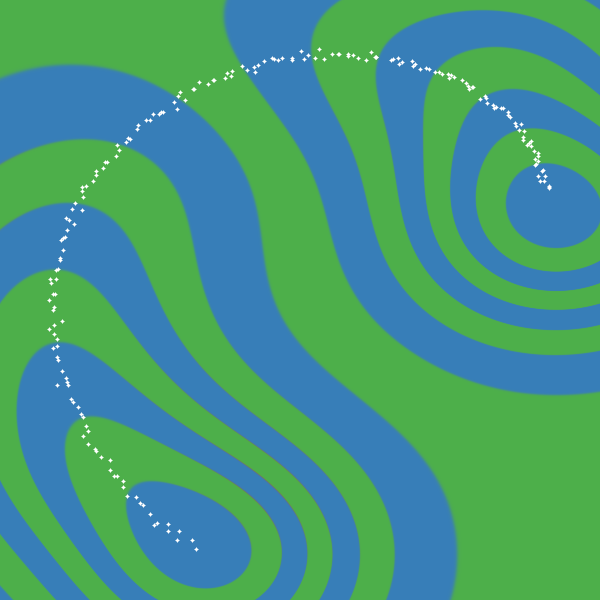
\includegraphics[width=0.45\columnwidth]{\deeplimitsfiguresdir/hidden_good} &
\begin{tikzpicture}[pile/.style={thick, ->, >=stealth'}]
    \node[anchor=south west,inner sep=0] at (0,0) {
    	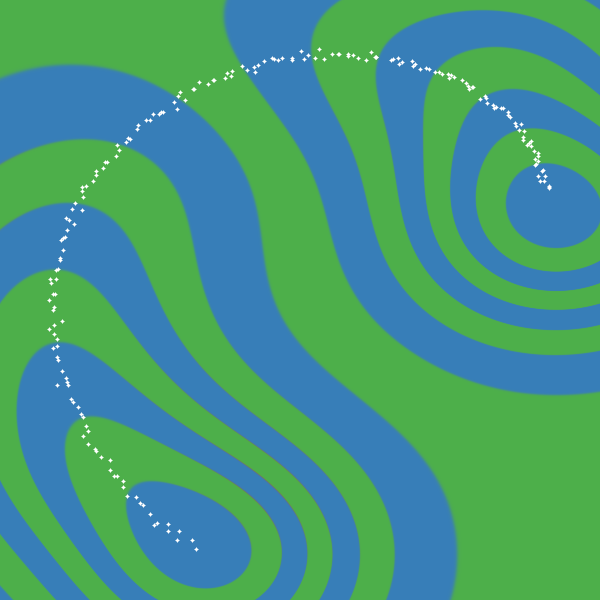
\includegraphics[clip, trim = 0cm 12cm 0cm 0.0cm, width=0.6\columnwidth]{\deeplimitsfiguresdir/hidden_good}
    };
    \coordinate (D) at (1.6,1.5);
    \coordinate (Do) at (2.5, 0.8);
    \coordinate (Dt) at (3,3);
    
    \draw[pile] (D) -- (Dt) node[above, text width=5em] { tangent };
    \draw[pile] (D) -- (Do) node[right, text width=5em] { orthogonal };
\end{tikzpicture}
%A noise-tolerant representation  of \\ a one-dimensional manifold (white)
%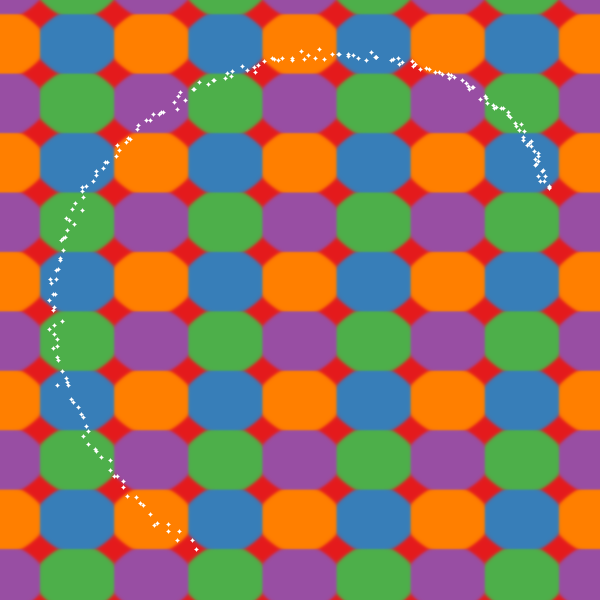
\includegraphics[clip, trim = 0cm 12cm 0cm 0.0cm, width=0.9\columnwidth]{\deeplimitsfiguresdir/hidden_bad} \\
%b) A na\"{i}ve representation (colors) \\ of a one-dimensional manifold (white)
%\end{tabular}
\caption[Desirable properties of representations of manifolds]
{Representing a 1-D data manifold.
%A representation is a function mapping the input space to some set of outputs.
Colors are a function of the computed representation of the input space.
The representation (blue \& green) varies in directions tangent to the data manifold (white), preserving information for later layers. 
The representation changes little in directions orthogonal to the manifold, making it robust to noise in those directions.
%, and reducing the number of parameters needed to represent a datapoint.
%Representation b) changes in all directions, preserving potentially useless information.}% The representation on the right might be useful if the data were spread out in over plane.
}
\label{fig:hidden}
\end{figure}

As in \citet{rifai2011contractive}, we characterize the representational properties of a function by the singular value spectrum of the Jacobian.
The number of relatively large singular values of the Jacobian roughly correspond to the number of directions in data-space in which the representation varies.
%
\newcommand{\spectrumpic}[1]{
\includegraphics[trim=4mm 1mm 4mm 2.5mm, clip, width=0.475\columnwidth]{\deeplimitsfiguresdir/spectrum/layer-#1}}%
\begin{figure}
\centering
\begin{tabular}{ccc}
& 2 Layers & 6 Layers \\
\begin{sideways} { \quad Normalized singular value} \end{sideways} & \hspace{-0.2in} \spectrumpic{2} & \hspace{-0.1in} \spectrumpic{6} \\
 & { Singular value index} & { Singular value index}
\end{tabular}
\caption[Distribution of singular values of the Jacobian of a deep \sgp{}]
{%The normalized singular value spectrum of the Jacobian of a deep \gp{} warping $\Reals^5 \to \Reals^5$.
The distribution of normalized singular values of the Jacobian of a function drawn from a 5-dimensional deep \gp{} prior 25 layers deep~(\emph{Left}) and 50 layers deep~(\emph{Right}).
As nets get deeper, the largest singular value tends to become much larger than the others.
This implies that with high probability, these functions vary little in all directions but one, making them insuitable for computing representations of manifolds of more than one dimension.
%As depth increases, the distribution on singular values also becomes heavy-tailed.
}
\label{fig:deep_spectrum}
\end{figure}%
%
\begin{figure}%
\centering
\begin{tabular}{cc}
No transformation: $p(\vx)$ & 1 Layer: $p \left( \vf^{(1)}(\vx) \right)$ \\
\gpdrawbox{1} & \gpdrawbox{2} \\
4 Layers: $p \left( \vf^{(1:4)}(\vx) \right)$ & 6 Layers: $p \left( \vf^{(1:6)}(\vx) \right)$ \\
\gpdrawbox{4} & \gpdrawbox{6}
\end{tabular}
\caption[Points warped by a draw from a deep \sgp{}]
{Points warped by a function drawn from a deep \gp{} prior.
\emph{Top left:} Points drawn from a 2-dimensional Gaussian distribution, color-coded by their location.
\emph{Subsequent panels:} Those same points, successively warped by compositions of functions drawn from a \gp{} prior.
As the number of layers increases, the density concentrates along one-dimensional filaments.
Warpings using random finite neural networks exhibit the same pathology, but also tend to concentrate density into 0-dimensional manifolds (points) due to saturation of the hidden units.}
\label{fig:filamentation}
\end{figure}%
%
\Cref{fig:deep_spectrum} shows the singular value spectrum for 5-dimensional deep GPs of different depths
\footnote{\citet{rifai2011contractive} analyzed the Jacobian at location of the training points, but because the priors we are examining are stationary, the distribution of the Jacobian is identical everywhere.}.
As the net gets deeper, the largest singular value dominates, implying there is usually only one effective degree of freedom in the representations being computed.

\Cref{fig:filamentation} demonstrates a related pathology that arises when composing functions to produce a deep density model.
The density in the observed space eventually becomes locally concentrated onto one-dimensional manifolds, or \emph{filaments}.
This again suggests that, when the width of the network is relatively small, deep compositions of independent functions are unsuitable for modeling manifolds whose underlying dimensionality is greater than one.

%for file in `ls`; do convert $file $file; done
\newcommand{\mappic}[1]{ \includegraphics[width=0.475\columnwidth]{\deeplimitsfiguresdir/map/latent_coord_map_layer_#1} } 
\newcommand{\mappiccon}[1]{ \includegraphics[width=0.475\columnwidth]{\deeplimitsfiguresdir/map_connected/latent_coord_map_layer_#1} }
\begin{figure}
\centering
\begin{tabular}{cc}
\hspace{-0.15in} Identity Map: $\vy = \vx$ &
\hspace{-0.15in} 1 Layer: $\vy = \vf^{(1)}(\vx)$ \\
\hspace{-0.15in} \mappic{0} & \mappic{1} \\
\hspace{-0.15in} 10 Layers: $\vy = \vf^{(1:10)}(\vx)$ &
\hspace{-0.15in} 40 Layers: $\vy = \vf^{(1:40)}(\vx)$ \\
\hspace{-0.15in} \mappic{10} & \mappic{40}
\end{tabular}
\caption[Visualization of a feature map drawn from a deep \sgp{}]
{A vizualization of the feature map implied by a function $\vf$ drawn from a deep \gp{}.
Colors are a function of the 2D representation $\vy = \vf(\vx)$ that each point is mapped to. % by the deep function. %that each point is mapped to after being warped by a deep \gp{}.
The number of directions in which the color changes rapidly corresponds to the number of large singular values in the Jacobian.
Just as the densities in \cref{fig:filamentation} became locally one-dimensional, there is usually only one direction that one can move $\vx$ in locally to change $\vy$.
This means that $\vf$ is unlikely to be a suitable representation for decision tasks that depend on more than one aspect of $\vx$.  Also note that the overall shape of the mapping remains the same as the number of layers increase.
For example, the roughly circular shape remains in the top-left corner even after 40 independent warpings.}
\label{fig:deep_map}
\end{figure}
%
To visualize this pathology in another way, \cref{fig:deep_map} illustrates a color-coding of the representation computed by a deep \gp{}, evaluated at each point in the input space.
After 10 layers, we can see that locally, there is usually only one direction that one can move in $\vx$-space in order to change the value of the computed representation, or to cross a decision boundary.
This means that such representations are likely to be unsuitable for decision tasks that depend on more than one property of the input.

To what extent are these pathologies present in the types of neural networks commonly used in practice?
In simulations, we found that for deep functions with a fixed hidden dimension $D$, the singular value spectrum remained relatively flat for hundreds of layers as long as $D > 100$.
Thus, these pathologies are unlikely to severely effect the relatively shallow, wide networks most commonly used in practice.





\section{Fixing the pathology}
\label{sec:fix}

As suggested by \citet[chapter 2]{neal1995bayesian}, we can fix the pathologies exhibited in figures \cref{fig:filamentation} and \ref{fig:deep_map} by simply making each layer depend not only on the output of the previous layer, but also on the original input $\vx$.  
We refer to these models as \emph{input-connected} networks, and denote deep functions having this architecture with the subscript $C$, as in $f_C(\vx)$.
Formally, this functional dependence can be written as
\begin{align}
\vf_C^{(1:L)}(\vx) = \vf^{(L)} \left( \vf_C^{(1:L-1)}(\vx), \vx \right), \quad \forall L
\end{align}
%
\Cref{fig:input-connected} shows a graphical representation of the two connectivity architectures.

\begin{figure}[h]%
\def\nodeseptwo{1.9cm}%
\def\nodesize{.35cm}%
\def\numhiddentwo{3}%
\centering
\begin{tabular}{ccc}
a) Standard \MLP{} connectivity & &
b) Input-connected architecture\\
\hspace{-4mm}
\begin{tikzpicture}[draw=black!80]
    \tikzstyle{neuron}=[circle,minimum size=17pt, draw = black!80, fill = white, thick]
    \tikzstyle{input neuron}=[neuron, fill=green!50];
    \tikzstyle{output neuron}=[neuron, fill=red!50];
    \tikzstyle{hidden neuron}=[neuron, fill=blue!50];
    \tikzstyle{pile} =[thick, ->, >=stealth', shorten <=7pt, shorten >=8pt];

    % Define the input layer node
    \coordinate (I) at (0, 0);

    % Define the hidden layer nodes
    \foreach \name / \y in {1,...,\numhiddentwo} {
        \coordinate (H-\name) at (\nodeseptwo*\y, 0);
    }

    \path[pile] (I) edge (H-1) {};
    % Connect every node            
    \foreach \name in {2,...,\numhiddentwo} {
	 	\pgfmathsetmacro\hindex{\name - 1}
		\path[pile] (H-\hindex) edge (H-\name) {};
    }

    \draw (I) node[neuron] {};
    \draw (I) node[below = 0.5cm]  {$\vx$};

    % Draw the hidden layer nodes
    \foreach \name / \y in {1,...,\numhiddentwo} {
		\draw (H-\name) node[neuron]  {};
        \draw (H-\name) node[below = 0.34cm] {$\vf^{(\y)}(\vx)$};
    }
\end{tikzpicture} &
\hspace{0.5cm} &
\begin{tikzpicture}[draw=black!80]
    \tikzstyle{neuron}=[circle,minimum size=17pt, draw = black!80, fill = white, thick]
    \tikzstyle{input neuron}=[neuron, fill=green!50];
    \tikzstyle{output neuron}=[neuron, fill=red!50];
    \tikzstyle{hidden neuron}=[neuron, fill=blue!50];
    \tikzstyle{pile} =[thick, ->, >=stealth', shorten <=7pt, shorten >=8pt];

    % Define the input layer node
    \coordinate (I) at (0, 0);

    % Define the hidden layer nodes
    \foreach \name / \y in {1,...,\numhiddentwo} {
        \coordinate (H-\name) at (\nodeseptwo*\y, 0);
    }

    % Connect every node            
    \path[pile] (I) edge (H-1) {};
    \foreach \name in {2,...,\numhiddentwo} {
		\pgfmathsetmacro\hindex{\name - 1}
		\path[pile] (H-\hindex) edge (H-\name) {};
        \path[pile] (I) edge [bend left] (H-\name) {};
    }

    \draw (I) node[neuron] {};
    \draw (I) node[below = 0.5cm]  {$\vx$};

    % Draw the hidden layer nodes
    \foreach \name / \y in {1,...,\numhiddentwo} {
		\draw (H-\name) node[neuron]  {};
       	\draw (H-\name) node[below = 0.34cm] {$\vf_C^{(\y)}(\vx)$};
    }
\end{tikzpicture}
\end{tabular}
\caption[Two different architectures for deep neural networks]
{Two different architectures for deep neural networks.
\emph{Left:} The standard architecture connects each layer's outputs to the next layer's inputs.
\emph{Right:} The input-connected architecture also connects the original input $\vx$ to each layer.}
\label{fig:input-connected}
\end{figure}%

Similar connections between non-adjacent layers can also be found the primate visual cortex \citep{maunsell1983connections}.
Visualizations of the resulting prior on functions are shown in \cref{fig:deep_draw_1d_connected,fig:no_filamentation,fig:deep_map_connected}.


\begin{figure}[h]
\centering
\setlength{\tabcolsep}{1.5pt}
\begin{tabular}{ccccc}
& 1 Layer & 2 Layers & 5 Layers & 10 Layers \\
\raisebox{0.6cm}{\rotatebox{90}{$f_C^{(1:L)}(x)$}} &
\onedsamplepiccon{1} &
\onedsamplepiccon{2} &
\onedsamplepiccon{5} &
\onedsamplepiccon{10} \\[-3pt]
 & $x$ & $x$ & $x$ & $x$
\end{tabular}
\caption[A draw from a 1D deep \sgp{} prior with each layer connected to the input]
{A draw from a 1D deep \gp{} prior with each layer connected to the input.
The $x$-axis is the same for all plots.
Even after many layers, the functions remain relatively smooth in some regions, while varying rapidly in other regions.
Compare to standard-connectivity deep \gp{} draws shown in \cref{fig:deep_draw_1d}.}
\label{fig:deep_draw_1d_connected}
\end{figure}
%
\newcommand{\gpdrawboxcon}[1]{
\setlength\fboxsep{0pt}
\hspace{-0.2in} 
\fbox{
\includegraphics[width=0.464\columnwidth]{\deeplimitsfiguresdir/deep_draws_connected/deep_sample_connected_layer#1}
}}
%
\begin{figure}
\centering
\begin{tabular}{cc}
3 Connected layers: $p \left( \vf_C^{(1:3)}(\vx) \right)$ & 6 Connected layers: $p \left( \vf_C^{(1:6)}(\vx) \right)$ \\
\gpdrawboxcon{3} &
\gpdrawboxcon{6}
\end{tabular}
\caption[Points warped by a draw from an input-connected deep \sgp{}]
{Points warped by a draw from a deep \sgp{} with each layer connected to the input $\vx$.
%\emph{Top left:} Points drawn from a 2-dimensional Gaussian distribution, color-coded by their location.
%\emph{Subsequent panels:} Those same points, successively warped by functions drawn from a \gp{} prior.
As depth increases, the density becomes more complex without concentrating only along one-dimensional filaments.}
\label{fig:no_filamentation}
\end{figure}
%
\begin{figure}
\centering
\newcommand{\spectrumpiccon}[1]{
\includegraphics[trim=4mm 1mm 4mm 2.5mm, clip, width=0.475\columnwidth]{\deeplimitsfiguresdir/spectrum/con-layer-#1}} 
\begin{tabular}{ccc}
 & 25 layers &  50 layers \\
\hspace{-0.5cm} \begin{sideways} {\scriptsize \quad Normalized singular value} \end{sideways} & \hspace{-0.2in} \spectrumpiccon{25} & \hspace{-0.16in} \spectrumpiccon{50} \\
 & {\scriptsize Singular value number} & {\scriptsize Singular value number}
\end{tabular}
\caption[Distribution of singular values of an input-connected deep \sgp{}]
{The distribution of singular values drawn from 5-dimensional input-connected deep \gp{} priors, 25 layers deep (\emph{Left}) and 50 layers deep (\emph{Right}).
Compared to the standard architecure, the singular values are more likely to remain the same size as one another, meaning that the model outputs are more often sensitive to several directions of variation in the input.}
\label{fig:good_spectrum}
\end{figure}
%
%
\begin{figure}
\centering
\begin{tabular}{cc}
\hspace{-0.15in} Identity map: $\vy = \vx$ &
\hspace{-0.15in} 2 Connected layers: $\vy = \vf^{(1:2)}(\vx)$ \\
\hspace{-0.15in} \mappic{0} & \mappiccon{2} \\
\hspace{-0.15in} 10 Connected layers: $\vy = \vf^{(1:10)}(\vx)$ &
\hspace{-0.15in} 20 Connected layers: $\vy = \vf^{(1:20)}(\vx)$ \\
\hspace{-0.15in} \mappiccon{10} & \mappiccon{20}
\end{tabular}
\caption[Feature map of an input-connected deep \sgp{}]
{The feature map implied by a function $\vf$ drawn from a deep \gp{} prior with each layer connected to the input $\vx$, visualized at various depths.
Compare to the map shown in \cref{fig:deep_map}.
%Just as the densities in \cref{fig:no_filamentation} remained locally two-dimensional even after many warpings, 
In the mapping shown here there are sometimes two directions that one can move locally in $\vx$ to in order to change the value of $\vf(\vx)$.
This means that the input-connected prior puts mass on a greater variety of types of representations, some of which depend on all aspects of the input.
}
\label{fig:deep_map_connected}
\end{figure}


The Jacobian of an input-connected deep function is defined by the recurrence
%
\newcommand{\sbi}[2]{\left[ \! \begin{array}{c} #1 \\ #2 \end{array} \! \right]} 
%\newcommand{\sbi}[2]{\left[ #1 \quad \!\! #2 \right]} 
\begin{align}
{J_C^{(1:L)} = J^{(L)} \sbi{ J_C^{(1:L-1)}}{I_D}}.
\end{align}
%
%So the entire Jacobian has the form:
%
%\begin{align}
%J^{1:L}(x) = J^L \sbi{ J^{L-1} \sbi{ \dots J^{4} \sbi{ J^{3} \sbi{ J^2 J^1 }{ I_D }}{ I_D } \dots }{ I_D \\ %\vdots }}{ I_D}
%\end{align}
%
where $I_D$ is a $D$-dimensional identity matrix.
In the case of a deep \gp{}, the input-connected Jacobian is still a product of independent Gaussian matrices.
\Cref{fig:good_spectrum} shows that with this architecture, even 50-layer deep \gp{}s have well-behaved singular value spectra.

The pathology examined in this section is an example of the sort of analysis made possible by a well-defined prior on functions.
%As explained in \cref{sec:relating}, \gp{}s are examples of a particular limit of Bayesian neural networks.
The figures and analysis done in this section could be done using Bayesian neural networks with finite numbers of nodes, but would be more difficult.
In particular, care would need to be taken to ensure that the networks do not produce degenerate mappings due to saturation of the hidden units.





\section{Deep kernels}
\label{sec:deep_kernels}

\cite{ bengio2006curse} showed that kernel machines have limited generalization ability when they use ``local'' kernels such as the squared-exp.
However, as we saw in \cref{ch:kernels,ch:grammar,ch:additive}, structured, non-local kernels can 
%be constructed through addition and multiplication which 
allow extrapolation.
Another way to build non-local kernels is by composing fixed feature maps, creating \emph{deep kernels}.
This section builds on the work of \citet{cho2009kernel}, who derived several kinds of deep kernels by applying multiple layers of feature mappings.

To return to an example given in \cref{sec:expressing-symmetries}, periodic kernels can be viewed as a 2-layer-deep kernel, in which the first layer maps $x \rightarrow [\sin(x), \cos(x)]$, and the second layer maps through basis functions corresponding to the \humble{SE} kernel.

%In addition to analyzing \MLP{}s with random weights, we can also analyze fixed feature mappings with different connectivity architectures.
 
%We can construct other useful kernels by composing fixed feature maps several times, creating deep kernels.


%Given a kernel $k_1(\vx, \vx') = \hPhi(\vx) \tra \hPhi(\vx')$, 
In principle, we can compose the implicit feature maps of any two kernels $k_a$ and $k_b$ to get a new kernel, which we'll denote by $\left( k_b \circ k_a \right)$:
%
\begin{align}
k_a(\vx, \vx') & = \hPhi_a(\vx) \tra \hPhi_a(\vx') \\
k_b(\vx, \vx') & = \hPhi_b(\vx) \tra \hPhi_b(\vx') \\
\left( k_b \circ k_a \right)(\vx, \vx') & = k_b \left(\hPhi_a(\vx), \hPhi_a(\vx') \right) 
 = \left[ \hPhi_b \left( \hPhi_a(\vx) \right)\right] \tra \hPhi_b \left(\hPhi_a(\vx') \right)
\end{align}
%
However, this composition might not always have a closed form if the number of hidden features of either kernel is infinite.

Fortunately, composing the squared-exp (\kSE{}) kernel with the implicit mapping given by any other kernel has a simple closed form.
If $k(\vx, \vx') = \hPhi(\vx)\tra \hPhi(\vx')$, then
%, this composition operation has a closed form for any starting kernel:% for any set of starting features $\hPhi_n(\vx)$:
%
\begin{align}
%k_1(\vx, \vx') & = \exp \left( -\frac{1}{2} ||\vx - \vx'||_2^2 \right) \\
\left( \kSE \circ k \right) \left( \vx, \vx' \right) & = k_{SE} \big( \hPhi(\vx), \hPhi(\vx') \big) \\
%& = \left( \hPhi^{SE} \left(\hPhi^{1}(\vx) \right) \right) \tra \hPhi^{SE} \left( \hPhi^{1}(\vx') \right) \\
& = \exp \left( -\frac{1}{2} || \hPhi(\vx) - \hPhi(\vx')||_2^2 \right) \\
%k_{n+1}(\vx, \vx') 
%& = \exp \left( -\frac{1}{2} \sum_i \left[ \hphi_n^{(i)}(\vx) - \hphi_n^{(i)}(\vx') \right]^2 \right) \\
& = \exp\left ( -\frac{1}{2} \left[ \hPhi(\vx) \tra \hPhi(\vx) - 2 \hPhi(\vx) \tra \hPhi(\vx') + \hPhi(\vx') \tra \hPhi(\vx') \right] \right)  \\
%k_2(\vx, \vx') & = \exp \left( -\frac{1}{2} \left[ \sum_i \hphi_i(\vx)^2 - 2 \sum_i \hphi_i(\vx) \hphi_i(\vx') + \sum_i \hphi_i(\vx')^2 \right] \right) \\
%k_{n+1}(\vx, \vx') 
& = \exp \left( -\frac{1}{2} \big[ k(\vx, \vx) - 2 k(\vx, \vx') + k(\vx', \vx') \big] \right) \; .
%k_{n+1}(\vx, \vx') 
%& = \exp \left( k_1(\vx, \vx') - 1 \right) \qquad \textnormal{(if $k_1(\vx, \vx) = 1$)} \nonumber
\end{align}
%
%\begin{figure}
%\centering
%\begin{tabular}{ccc}
%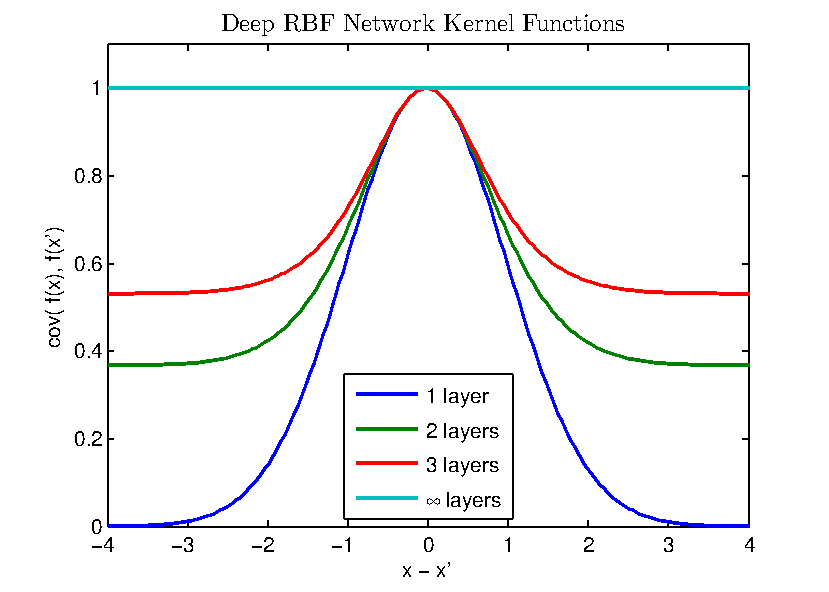
\includegraphics[width=0.5\columnwidth, clip, trim = 0cm 0cm 0cm 0.61cm]{\deeplimitsfiguresdir/deep_kernel} &
%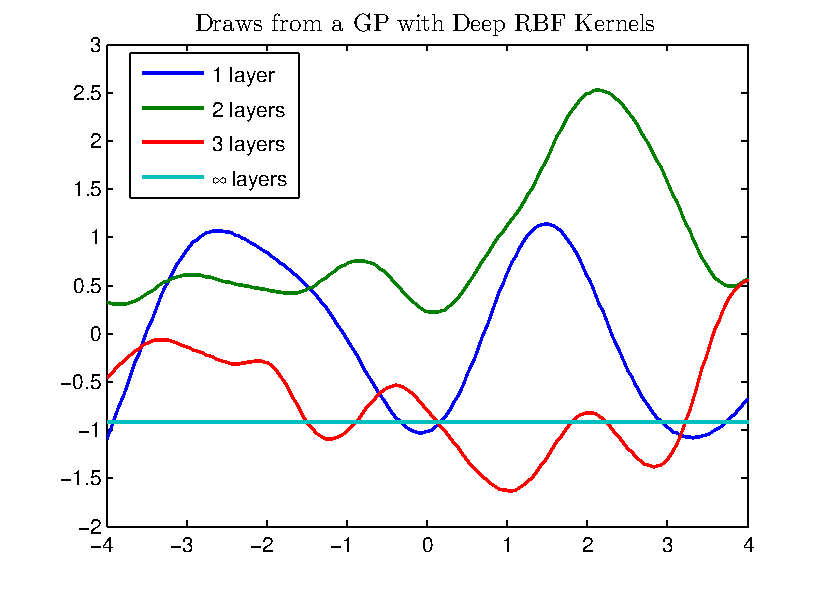
\includegraphics[width=0.5\columnwidth, clip, trim = 0cm 0cm 0cm 0.61cm]{\deeplimitsfiguresdir/deep_kernel_draws} \\
%Kernel derived from iterated feature transforms & Draws from the corresponding kernel
%\end{tabular}
%\caption{A degenerate kernel produced by repeatedly applying a feature transform.}
%\label{fig:deep_kernel}
%\end{figure}
%
%Thus, if $k_1(x,y) = e^{-||x - y||2}$, then the two-layer kernel is simply $k_2(x,y) = e^{k_1(x, y) - 1}$.  This formula is true for every layer: $k_{n+1}(x,y) = e^{k_n(x, y) - 1}$.
%
%Note that nothing in this derivation depends on details of $k_n$, except that $k_n( \vx, \vx) = 1$.
%Note that this result holds for any base kernel $k_n$, as long as $k_n( \vx, \vx) = 1$.
%  Because this is true for $k_2$ as well, this recursion holds in general, and we have that $k_{n+1}(x,y) = e^{k_n(x, y) - 1}$.  
This formula lets expresses the composed kernel $(\kSE \circ k)$ exactly in terms of evaluations of the original kernel $k$.

\subsection{Infinitely deep kernels}
What happens when we repeatedly compose feature maps many times, starting with the squared-exp kernel?
If the output variance of the \kSE{} is normalized to ${k(\vx,\vx) = 1}$, then the infinite limit of composition with \kSE{} converges to ${\left(\kSE \circ \kSE \circ \kSE \circ \ldots \circ \kSE\right)(\vx,\vx') = 1}$ for all pairs of inputs.
A constant covariance corresponds to a prior on constant functions ${f(\vx) = c}$.

%Figure \ref{fig:deep_kernel_connected} shows this kernel at different depths, including the degenerate limit.  
%
%One interpretation of why repeated feature transforms lead to this degenerate prior is that each layer can only lose information about the previous set of features.  
%In the limit, the transformed features contain no information about the original input $\vx$.  Since the function doesn't depend on its input, it must be the same everywhere.

%\subsubsection{A non-degenerate construction}

As above, we can overcome this degeneracy by connecting the input $\vx$ to each layer.
To do so, we concatenate the composed feature vector at each layer, $\hPhi^{(1:\ell)}(\vx)$, with the input vector $\vx$, to produce an input-connected deep kernel $k_C^{(1:L)}$, defined by:
%
\begin{align}
%k_1(\vx, \vx') & = \exp \left( -\frac{1}{2} ||\vx - \vx'||_2^2 \right) \\
k_C^{(1:\ell + 1)}(\vx, \vx')
& = \exp \left( -\frac{1}{2} \left|\left| 
\left[ \! \begin{array}{c} \hPhi^{(1:\ell)}(\vx) \\ \vx \end{array} \! \right] - 
\left[ \! \begin{array}{c} \hPhi^{(1:\ell)}(\vx') \\ \vx' \end{array} \! \right] \right| \right|_2^2 \right) \\
%k_{n+1}(\vx, \vx') 
%& = \exp \left( -\frac{1}{2} \sum_i \left[ \hphi_i(\vx) - \hphi_i(\vx') \right]^2 -\frac{1}{2} || \vx - \vx' ||_2^2 \right) \\
%k_{n+1}(\vx, \vx') & = \exp\left ( -\frac{1}{2} \sum_i \left[ \hphi_i(\vx)^2 - 2 \hphi_i(\vx) \hphi_i(\vx') + \hphi_i(\vx')^2 \right]  -\frac{1}{2} || \vx - \vx' ||_2^2 \right) \\
%k_2(\vx, \vx') & = \exp \left( -\frac{1}{2} \left[ \sum_i \hphi_i(\vx)^2 - 2 \sum_i \hphi_i(\vx) \hphi_i(\vx') + \sum_i \hphi_i(\vx')^2 \right] \right) \\
%k_2(\vx, \vx') & = \exp \left( -\frac{1}{2} \left[ k_1(\vx, \vx) - 2 k_1(\vx, \vx') + k_1(\vx', \vx') \right] \right) \\
%k_{n+1}(\vx, \vx') 
%& = \exp \left( k_n(\vx, \vx') - 1 -\frac{1}{2} || \vx - \vx' ||_2^2 \right)
& = \exp \Big( -\frac{1}{2} \big[ k_C^{(1:\ell)}(\vx, \vx) - 2 k_C^{(1:\ell)}(\vx, \vx') 
 + k_C^{(1:\ell)}(\vx', \vx') {\color{black} - || \vx - \vx' ||_2^2} \big] \Big) \nonumber
\end{align}
%
Starting with the squared-exp kernel, this repeated mapping satisfies
\begin{align}
k_C^{(1:\infty)}(\vx, \vx') - \log \left( k_C^{(1:\infty)}(\vx, \vx') \right) = 1 + \frac{1}{2} || \vx - \vx' ||_2^2 \,.
\end{align}
%
\begin{figure}
\centering
\begin{tabular}{cc}
Input-connected deep kernels & Draws from corresponding \gp{}s \\
\hspace{-0.3cm}
\rotatebox{90}{$\qquad \qquad k(x, x')$}
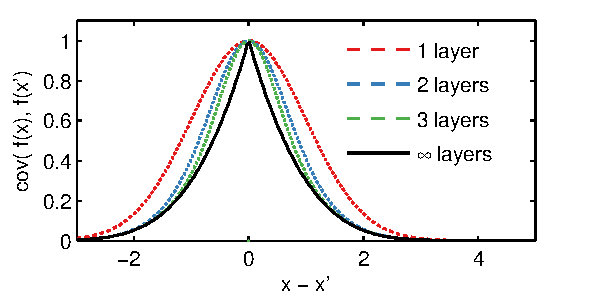
\includegraphics[width=0.465\columnwidth, clip, trim = 1.3cm 0.4cm 0.9cm 0.3cm]{\deeplimitsfiguresdir/deep_kernel_connected} &
\hspace{-0.3cm}
\rotatebox{90}{$\qquad \qquad f(x)$}
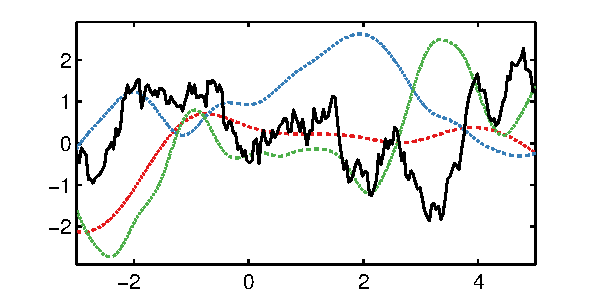
\includegraphics[width=0.44\columnwidth, clip, trim = 1.29cm 0.1cm 0.9cm 0.35cm]{\deeplimitsfiguresdir/deep_kernel_connected_draws} \\
$ x - x'$ &  $ x - x'$
\end{tabular}
\caption[Infinitely deep kernels]{
\emph{Left:} Input-connected deep kernels of different depths.
By connecting the input $\vx$ to each layer, the kernel can still depend on its input even after arbitrarily many layers of composition.
\emph{Right:} Draws from \gp{}s with deep input-connected kernels.}
\label{fig:deep_kernel_connected}
\end{figure}
%
The solution to this recurrence has no closed form, but for one input dimension, has a similar shape to the Ornstein-Uhlenbeck covariance ${\OU(x,x') = \exp( -|x - x'| )}$ but with lighter tails.
%
Samples from a \gp{} prior with this kernel are not differentiable, and are locally fractal.
\Cref{fig:deep_kernel_connected} shows this kernel at different depths, as well as samples from the resulting \gp{} priors.
%\item This kernel has smaller correlation than the squared-exp everywhere except at $\vx = \vx'$.  
%\item The tails have the same form as the squared-exp.

We can also consider two related connectivity architectures: one in which each layer is connected to the output layer, and another in which every layer is connected to all subsequent layers.
It is easy to show that in the limit of infinite depth of composing \kSE{} kernels, both these architectures converge to $k(\vx, \vx') = \delta( \vx, \vx' )$, the white noise kernel.



%\subsection{A fully-connected kernel}
%However, connecting every layer to every subsequent layer leades to a pathology:
%\begin{align}
%k_1(\vx, \vx') & = \exp \left( -\frac{1}{2} ||\vx - \vx'||_2^2 \right) \\
%k_{n+1}(\vx, \vx') & = \exp \left( -\frac{1}{2} \left|\left| \left[ \! \begin{array}{c} \hPhi_n(\vx) \\ \hPhi_{n-1}(\vx') \end{array} \! \right]  - \left[ \! \begin{array}{c} \hPhi_n(\vx') \\ \hPhi_{n-1}(\vx') \end{array} \! \right] \right| \right|_2^2 \right) \\
%k_{n+1}(\vx, \vx') & = \exp \left( -\frac{1}{2} \sum_i \left[ \hphi^{(i)}_n(\vx) - \hphi^{(i)}_n(\vx') \right]^2 -\frac{1}{2} \sum_i \left[ \hphi^{(i)}_{n-1}(\vx) - \hphi^{(i)}_{n-1}(\vx') \right]^2 \right)\\
%k_{n+1}(\vx, \vx') & = \exp\left ( -\frac{1}{2} \sum_i \left[ \hphi_i(\vx)^2 - 2 \hphi_i(\vx) \hphi_i(\vx') + \hphi_i(\vx')^2 \right]  -\frac{1}{2} || \vx - \vx' ||_2^2 \right) \\
%k_2(\vx, \vx') & = \exp \left( -\frac{1}{2} \left[ \sum_i \hphi_i(\vx)^2 - 2 \sum_i \hphi_i(\vx) \hphi_i(\vx') + \sum_i \hphi_i(\vx')^2 \right] \right) \\
%k_2(\vx, \vx') & = \exp \left( -\frac{1}{2} \left[ k_1(\vx, \vx) - 2 k_1(\vx, \vx') + k_1(\vx', \vx') \right] \right) \\
%k_{n+1}(\vx, \vx') & = \exp \left( k_n(\vx, \vx') - 1 \right) \exp \left( k_{n-1}(\vx, \vx') - 1 \right)
%k_{n+1}(\vx, \vx') & = \prod_{i=1}^n \prod_{j=1}^i \exp \left( k_i(\vx, \vx') - 1 \right)
%\end{align}
%Which has the solution $k_\infty = \delta( \vx = \vx' )$, a white noise kernel.


%\subsection{Connecting every layer to the end}
%There is a fourth possibilty (suggested by Carl), of connecting every layer to the output:
%\begin{align}
%k_n(\vx, \vx') & = \exp \left( -\frac{1}{2} || \hPhi_n(\vx) - \hPhi_n(\vx')||_2^2 \right) \\
%k_{n+1}(\vx, \vx') & = \exp \left( k_n(\vx, \vx') - 1 \right) \\
%k_{L}(\vx, \vx') & = \prod_{i=1}^L \exp \left( k_i(\vx, \vx') - 1 \right)
%\end{align}
%Which also has the solution $k_\infty = \delta( \vx = \vx' )$, a white noise kernel.


\subsection{When are deep kernels useful models?}

Kernels correspond to fixed feature maps, and so kernel learning is an example of implicit representation learning. %can compute %useful representations.
As we saw in \cref{ch:kernels,ch:grammar}, kernels can capture rich structure and can enable many types of generalization.
 %, such as affine invariance in images \citep{kondor2008group}.
%\cite{salakhutdinov2008using} used a deep neural network to learn feature transforms for kernels, which learn invariants in an unsupervised manner.
We believe that the relatively uninteresting properties of the deep kernels derived in this section simply reflect the fact that an arbitrary computation, even if it is ``deep'', is not likely to give rise to a useful representation unless combined with learning.
To put it another way, any fixed representation is unlikely to be useful unless it has been chosen specifically for the problem at hand.






\section{Related work}

\subsubsection{Deep Gaussian processs}
\citet[chapter 2]{neal1995bayesian} explored properties of arbitrarily deep Bayesian neural networks, including those that would give rise to deep \gp{}s.
He noted that infinitely deep random neural networks without extra connections to the input would be equivalent to a Markov chain, and therefore would lead to degenerate priors on functions.
He also suggested connecting the input to each layer in order to fix this problem.
Much of the analysis in this chapter can be seen as a more detailed investigation, and vindication, of these claims.

The first instance of deep \gp{}s being used in practice was \citep{lawrence2007hierarchical}, who presented a model called ``hierarchical \gplvm{}s'', in which time was mapped through a composition of multiple \gp{}s to produce observations.

%The term ``deep Gaussian processes'' first appeared in \citet{damianou2012deep}, where it referred to a latent variable model whose warping function was defined by a composition of \gp{}s.
The term ``deep Gaussian processes'' was first used by \citet{damianou2012deep}, who developed a variational inference method, analyzed the effect of automatic relevance determination, and showed that deep \gp{}S could learn with relatively little data.
%I propose that this model might be more clearly described as a ``deep \gplvm{}'', and that the term ``deep Gaussian process'' should be reserved for describing compositions of functions drawn from \gp{} priors.
%
They used the term ``deep \gp{}'' to refer both to supervised models (compositions of \gp{}s) and to unsupervised models (compositions of \gplvm{}s).
This conflation may be reasonable, since the activations of the hidden layers are themselves latent variables, even in supervised settings:
Depending on kernel parameters, each latent variable may or may not depend on the layer below.

In general, supervised models can also be latent-variable models.
For example, \citet{wang2012gaussian} investigated single-layer \gp{} regression models that had additional latent inputs.

\subsubsection{Nonparametric neural networks}
%Other Bayesian deep neural network models have been proposed by, for example, . % and Sum-product networks \cite{poon2011sum}  
\citet{adams2010learning} proposed a prior on arbitrarily deep Bayesian networks with an unknown and unbounded number of parametric hidden units in each layer.
Their architecture has connections only between adjacent layers, and so may be expected to have similar pathologies to those of deep \gp{}s as the number of layers increases.

\citet{wilson2012gaussian} introduced Gaussian process regression networks, which are defined as a matrix product of draws from \gp{}s priors, rather than a composition.
These networks have the form:
%The form of a \gprn{} is
%
\begin{align}
\vy(\vx) & = \vW^(\vx) \vf(\vx) \qquad \textnormal{with each} \; f_{d}, W_{d,j} \simiid \GPt{\vzero}{\kSE + \kWN} .
\end{align}
%
We can easily define a ``deep'' Gaussian process regression network:
%
\begin{align}
\vy(\vx) = \vW^{(3)}(\vx) \vW^{(2)}(\vx) \vW^{(1)}(\vx) \vf(\vx)
\end{align}
%
which repeatedly adds and multiplies functions drawn from \gp{}s, in contrast to deep \gp{}s, which repeatedly compose functions.
This prior on functions has a similar form to the Jacobian of a deep \gp{} (\cref{eq:jacobian-of-deep-gp}), and so might be amenable to a similar analysis to that of section \ref{sec:characterizing-deep-gps}.

%
%This model has a similar form to the Jacobian of deep \gp{}, (since each row of the Jacobian is jointly a \gp{} but with with a kernel given by \eqref{eq:deriv-kernel}) except that the Jacobian is evaluated at the output from previous layers:
%
%\begin{align}
%\vy(\vx) = J^3(\vf^2(\vx)) J^2(\vf^1(\vx)) J^1(\vx)
%\end{align}
%

\subsubsection{Information-preserving architectures}
Deep density networks \citep{rippel2013high} are constructed through a series of parametric warpings of fixed dimension, with penalty terms encouraging the preservation of information about lower layers.
This is another promising approach to fixing the pathology discussed in \cref{sec:formalizing-pathology}.

\subsubsection{Recurrent networks}
\citet{bengio1994learning} and \citet{pascanu2012understanding} analyze a related problem with gradient-based learning in recurrent networks, the ``exploding-gradients'' problem.
They note that in recurrent neural networks, the size of the training gradient can grow or shrink exponentially as it is back-propagated, making gradient-based training difficult.

\citet{hochreiter1997long} addressed the exploding-gradients problem by including hidden units designed to have stable gradients.

\subsubsection{Deep kernels}

The first systematic examination of deep kernels was done by \citet{cho2009kernel}, who derived closed-form composition rules for $\kSE$, polynomial, and arc-cosine kernels, and showed that deep arc-cosine kernels performed competitively in machine-vision applications when used in a \SVM{}.
%\citet{cho2012kernel} 

\citet{hermans2012recurrent} constructed deep kernels in a time-series setting, constructing kernels corresponding to infinite-width \emph{recurrent} neural networks.
They also proposed concatenating the implicit feature vectors from previous time-steps with the current inputs, resulting in an architecture analogous to the input-connected architecture proposed by \citet[chapter 2]{neal1995bayesian}.

\subsubsection{Analyses of deep learning}
\citet{montavon2010layer} performed a layer-wise analysis of deep networks, and noted that the performance of \MLP{}s degrades as the number of layers with random weights increases.

The experiments of \citet{saxe2011random} suggested that most of the performance of convolutional neural networks could be attributed to the architecture alone.
Later, \citet{saxedynamics} looked at the dynamics of gradient-based training methods in deep \emph{linear} networks as a tractable approximation to standard deep (nonlinear) neural networks.  




%\section{Discussion}


%\paragraph{Recursive learning method}
%Just as layer-wise unsupervised pre-training encourages the projection of the data into a representation with independent features in the higher layers, so does the procedure outlined here.  This is because the isotropic kernel does not penalize independence between different dimensions, only the number of dimensions.


\subsubsection{Source code}
Source code to produce all figures is available at \url{http://www.github.com/duvenaud/deep-limits}.
This code is also capable of producing visualizations of mappings such as \cref{fig:deep_map,fig:deep_map_connected} using neural nets instead of \gp{}s at each layer.


\section{Conclusions}

%In this work, we established a number of propositions which help us gain insight into the properties of very deep models, and allow making informed choices regarding their architecture.

This chapter demonstrated that well-defined priors allow explicit examination of the assumptions being made about functions being modeled by different neural network architectures.
As an example of the sort of analysis made possible this way, we attempted to gain insight into the properties of deep neural networks by characterizing the sorts of functions likely to be obtained under different choices of priors on compositions of functions.
%established a number of propositions which help us gain insight into the properties of very deep models, and allow making informed choices regarding their architecture.

%First, we identified equivalences between multi-layer perceptions and deep \gp{}s --- namely, that a deep \gp{} can be written as an \MLP{}s with a finite number of nonparametric hidden units, or as an \MLP{} with infinitely-many parametric hidden units.
First, we identified deep Gaussian processes as an easy-to-analyze model corresponding to multi-layer preceptrons with nonparametric activation functions.
%  We also showed several other connections between deep \MLP{}s and different Gaussian process models. %equivalences between multi-layer perceptions and deep \gp{}s --- namely, that a deep \gp{} can be written as an \MLP{}s with a finite number of nonparametric hidden units, or as an \MLP{} with infinitely-many parametric hidden units.
%
%Second, we characterized the derivatives and Jacobians of deep \gp{}s through products of independent Gaussian matrices. % can be characterized using random matrix theory, which we applied to establish results regarding the distribution over the Jacobian of the composition transformation. 
We then showed that representations based on repeated composition of independent functions exhibit a pathology where the representations becomes invariant to all but one direction of variation. % This leads to extremely restricted expressiveness of such deep models in the limit of increasing number of layers. 
Finally, we showed that this problem could be alleviated by connecting the input to each layer.
%proposed a way to alleviate this problem: connecting the input to each layer of a deep representation allows us to construct priors on deep functions that do not exhibit the information-capacity pathology.
%
We also examined properties of deep kernels, corresponding to arbitrarily many compositions of fixed features.
%Finally, we derived models obtained by performing dropout on Gaussian processes, finding a tractable approximation to exact dropout in \gp{}s.

Much recent work on deep networks has focused on weight initialization \citep{martens2010deep}, regularization \citep{lee2007sparse} and network architecture \citep{gens2013learning}.
%However, the interactions between these different design decisions can be complex and difficult to characterize.
%We propose to approach the design of deep architectures by examining the problem of assigning priors to nested compositions of functions.
% Although inference in fully Bayesian models is generally challenging, well-defined priors allow us to encode our beliefs into models in a data-independent way. 
If we can identify priors that give our models desirable properties, these in turn may suggest regularization, initialization, and architecture choices that also provide such properties.

Existing neural network practice also requires expensive tuning of model hyperparameters such as the number of layers, the size of each layer, and regularization penalties by cross-validation.
One advantage of deep \gp{}s is that the approximate marginal likelihood allows a principled method for automatically determining such model choices.




\outbpdocument{
%This will be ignored, it's just so that Gummi can find the bibliography.
\bibliographystyle{plainnat}
\bibliography{references.bib}
qwerty
}

